% ============================================================================
% MAIN.TEX - Master Document for GIS Services Proposal
% ============================================================================

% ============================================================================
% PREAMBLE - LaTeX Configuration for GIS Services Proposal
% ============================================================================

\documentclass[12pt,a4paper,oneside]{book}

% ============================================================================
% PACKAGES
% ============================================================================

% Core Packages
\usepackage[utf8]{inputenc}
\usepackage[T1]{fontenc}
\usepackage{lmodern}
\usepackage[margin=1in,top=1.2in,bottom=1.2in]{geometry}
\usepackage{setspace}
\onehalfspacing

% Color Scheme (Professional Dark Blue / Red / Orange)
\usepackage[dvipsnames,svgnames,x11names]{xcolor}
\definecolor{PrimaryBlue}{RGB}{0,51,102}      % Dark professional blue
\definecolor{SecondaryBlue}{RGB}{0,102,204}   % Medium blue
\definecolor{AccentGreen}{RGB}{220,53,69}     % Professional red (replaced green)
\definecolor{AccentRed}{RGB}{220,53,69}       % Professional red
\definecolor{AccentOrange}{RGB}{255,140,0}    % Dark orange
\definecolor{DarkGrey}{RGB}{51,51,51}         % Dark grey
\definecolor{LightGrey}{RGB}{240,240,240}     % Light grey
\definecolor{HeaderGrey}{RGB}{80,80,80}       % Header grey

% Typography & Styling
\usepackage{fancyhdr}
\usepackage{titlesec}
\usepackage{titletoc}
\usepackage[hidelinks]{hyperref}
\hypersetup{
    colorlinks=true,
    linkcolor=SecondaryBlue,
    citecolor=SecondaryBlue,
    urlcolor=SecondaryBlue,
    pdftitle={GIS Drone Services Proposal - Bangladesh},
    pdfauthor={Md Rakib Hasan},
    pdfsubject={Business Proposal},
    pdfkeywords={GIS, LiDAR, Photogrammetry, Bangladesh}
}

% Tables & Data
\usepackage{booktabs}
\usepackage{tabularx}
\usepackage{array}
\usepackage{multirow}
\usepackage{makecell}

% Graphics & Figures
\usepackage{graphicx}
\usepackage{tikz}
\usepackage{pgfplots}
\usepackage{float}
\usepackage{caption}
\usepackage{subcaption}
\usepackage{wrapfig}

% Data Visualization (pgfplots)
\pgfplotsset{compat=1.18}
\usepgfplotslibrary{groupplots}

% Lists & Formatting
\usepackage{enumitem}
\usepackage{amssymb}
\usepackage{amsmath}

% Bibliography
\usepackage[
    backend=biber,
    style=numeric-comp,
    sorting=nyt,
    hyperref=true
]{biblatex}
\addbibresource{references.bib}

% Watermark (Confidentiality) - REMOVED
% \usepackage{draftwatermark}
% Watermark removed - document is now official proposal

% Code Listings (if needed)
\usepackage{listings}
\lstset{
    basicstyle=\ttfamily\small,
    breaklines=true,
    breakatwhitespace=true,
    frame=single,
    backgroundcolor=\color{LightGrey}
}

% ============================================================================
% CUSTOM FORMATTING
% ============================================================================

% Chapter Styling
\titleformat{\chapter}[display]
    {\normalfont\huge\bfseries\color{PrimaryBlue}}
    {\chaptertitlename\ \thechapter}
    {20pt}
    {}
    [\vspace{15pt}\rule{\textwidth}{2pt}]

% Section Styling
\titleformat{\section}
    {\normalfont\Large\bfseries\color{SecondaryBlue}}
    {\thesection}
    {10pt}
    {}

% Subsection Styling
\titleformat{\subsection}
    {\normalfont\large\bfseries\color{DarkGrey}}
    {\thesubsection}
    {8pt}
    {}

% Subsubsection Styling
\titleformat{\subsubsection}
    {\normalfont\normalsize\bfseries\color{HeaderGrey}}
    {\thesubsubsection}
    {6pt}
    {}

% ============================================================================
% HEADER & FOOTER
% ============================================================================

\pagestyle{fancy}
\fancyhf{}

% Header
\fancyhead[L]{\small\textcolor{DarkGrey}{GIS Drone Services Proposal}}
\fancyhead[R]{\small\textcolor{DarkGrey}{Bangladesh 2026}}

% Footer
\fancyfoot[C]{\small\textcolor{DarkGrey}{\thepage}}
\fancyfoot[L]{\small\textcolor{DarkGrey}{Confidential}}
\fancyfoot[R]{\small\textcolor{DarkGrey}{February 2026}}

% Remove line
\renewcommand{\headrulewidth}{0.5pt}
\renewcommand{\headrule}{\color{SecondaryBlue}\hrule}
\renewcommand{\footrulewidth}{0.5pt}
\renewcommand{\footrule}{\color{SecondaryBlue}\hrule}

% ============================================================================
% CUSTOM COMMANDS
% ============================================================================

% Key Highlight Box
\newcommand{\highlight}[1]{
    \tcbox[
        on line,
        arc=3pt,
        colback=LightGrey,
        colframe=SecondaryBlue,
        boxrule=1pt
    ]{#1}
}

% Important Note Box
\usepackage{tcolorbox}
\newtcolorbox{importantbox}{
    colback=yellow!10,
    colframe=AccentGreen,
    boxrule=1pt,
    arc=3pt,
    left=10pt,
    right=10pt,
    top=8pt,
    bottom=8pt,
    fontupper=\small
}

% Table Header Style
\newcommand{\theader}[1]{\textbf{\textcolor{white}{\cellcolor{PrimaryBlue}#1}}}

% Figure Reference
\newcommand{\figref}[1]{Figure~\ref{#1}}
\newcommand{\tableref}[1]{Table~\ref{#1}}

% ============================================================================
% TABLE OF CONTENTS STYLING
% ============================================================================

\renewcommand{\contentsname}{\textcolor{PrimaryBlue}{\Large Table of Contents}}

% ============================================================================
% END OF PREAMBLE
% ============================================================================


\begin{document}

% ============================================================================
% TITLE PAGE
% ============================================================================

\begin{titlepage}
    \begin{center}
        \vspace*{2cm}

        % Logo Placeholder
        \textcolor{PrimaryBlue}{\rule{\textwidth}{3pt}}

        \vspace{1.5cm}

        {\Huge\bfseries\textcolor{PrimaryBlue}{
            GIS DRONE SERVICES PROPOSAL
        }}

        \vspace{0.5cm}

        {\Large\textcolor{SecondaryBlue}{
            Bangladesh LiDAR \& Photogrammetry Technology Initiative
        }}

        \vspace{3cm}

        \textcolor{DarkGrey}{\rule{0.8\textwidth}{1pt}}

        \vspace{2cm}

        {\large\textcolor{DarkGrey}{
            \textbf{Document Information}
        }}

        \vspace{1cm}

        \begin{tabular}{l l}
            \textbf{Prepared For:} & Startup GIS Company, Bangladesh \\
            \textbf{Version:} & 1.0 \\
            \textbf{Date:} & February 2026 \\
            \textbf{Status:} & Draft - Confidential \\
            \textbf{Geographic Focus:} & Bangladesh (4 Regions) \\
        \end{tabular}

        \vspace{2cm}

        {\large\textcolor{AccentGreen}{
            \textbf{Key Business Parameters}
        }}

        \vspace{1cm}

        \begin{tabular}{c | c | c}
            \hline
            \textbf{Initial Investment} & \textbf{Break-even} & \textbf{3-Yr Revenue} \\
            \hline
            BDT 100-125L & Month 10 & BDT 330.5L \\
            (USD 120-150K) & (Year 1) & \\
            \hline
        \end{tabular}

        \vspace{3cm}

        \textcolor{DarkGrey}{\rule{0.8\textwidth}{1pt}}

        \vspace{2cm}

        {\footnotesize\textcolor{DarkGrey}{
            \textit{This document contains proprietary and confidential information.} \\
            \textit{Unauthorized copying or distribution is strictly prohibited.}
        }}

        \vfill

        {\small\textcolor{DarkGrey}{
            Generated by Claude Code AI\\
            \textit{Proposal Builder}
        }}

    \end{center}
\end{titlepage}

% ============================================================================
% EXECUTIVE SUMMARY (Not a Chapter)
% ============================================================================

\cleardoublepage

\chapter*{Executive Summary}
\addcontentsline{toc}{chapter}{Executive Summary}

This proposal outlines the establishment of a premium GIS services company leveraging drone-mounted LiDAR and photogrammetry technology across Bangladesh. The startup will serve agriculture, government, real estate, and environmental sectors through data collection, processed analysis, custom applications, and consulting services.

\vspace{1cm}

\textcolor{SecondaryBlue}{\textbf{Key Business Parameters:}}

\begin{itemize}[noitemsep]
    \item \textbf{Business Model:} Startup (newly formed)
    \item \textbf{Initial Investment:} BDT 100+ lakhs (USD 120,000+)
    \item \textbf{Team Structure:} Core in-house + External consultants
    \item \textbf{Growth Target (Year 1-3):} 5 → 20 → 50+ projects
    \item \textbf{Competitive Edge:} Advanced LiDAR + ML integration technology
    \item \textbf{Revenue Streams:} Multi-model (projects, subscriptions, apps, consulting)
    \item \textbf{Break-even Timeline:} Month 10, Year 1
    \item \textbf{Expected 3-Year ROI:} 187\% (85-95\% IRR)
\end{itemize}

\vspace{1cm}

\begin{importantbox}
    \textbf{Opportunity:} Bangladesh has an emerging GIS services market with strong demand from agriculture, government, and real estate sectors. LiDAR technology remains relatively untapped compared to basic photogrammetry, presenting a unique market entry opportunity for early movers with advanced technology.
\end{importantbox}

\newpage

% ============================================================================
% TABLE OF CONTENTS
% ============================================================================

\tableofcontents

\newpage

% ============================================================================
% INCLUDE CHAPTERS
% ============================================================================

% Chapter 0: Detailed Competitive Landscape (NEW - INSERTED FIRST)
% ============================================================================
% CHAPTER 0: DETAILED COMPETITIVE LANDSCAPE & MARKET RESEARCH
% ============================================================================

\chapter*{Market Research: Competitive Landscape Analysis}
\addcontentsline{toc}{chapter}{Market Research: Competitive Landscape Analysis}

\section{Bangladesh GIS \& Drone Services Market - Current State}

This chapter provides detailed market research on existing GIS, drone, and LiDAR service providers currently operating in Bangladesh, based on comprehensive research conducted in February 2026.

\begin{importantbox}
    \textbf{Key Finding:} While Bangladesh has several drone survey companies, the market for LiDAR + Data Science integration remains largely untapped. This represents a significant market opportunity for a technology-forward startup.
\end{importantbox}

\section{Identified Competitors in Bangladesh}

\subsection{1. GeoTech Engineering Ltd. (Established Leader)}

\textbf{Company Profile:}
\begin{itemize}
    \item \textbf{Experience:} 23+ years in geotechnical and surveying engineering
    \item \textbf{Services:} Drone surveys, topographic mapping, LiDAR services
    \item \textbf{Specialization:} Land surveying, bored piles, soil testing, pile foundations
    \item \textbf{Geographic Coverage:} Bangladesh and Nepal
    \item \textbf{Website:} https://www.geotechengbd.com/
\end{itemize}

\textbf{Service Offerings:}
\begin{itemize}
    \item Digital Orthophotography/Orthomosaic Maps
    \item Digital Planimetric and Topographic Mapping
    \item Digital Terrain Models (DTM) and Digital Surface Models (DSM)
    \item Digital Aerial Triangulation
    \item 3D Texture Models
    \item Volumetric Analysis
    \item Environmental Monitoring
    \item LiDAR survey services
\end{itemize}

\textbf{Competitive Assessment:}
\begin{itemize}
    \item \textcolor{AccentGreen}{$\checkmark$ Strength:} Long-established reputation, comprehensive service portfolio
    \item \textcolor{AccentGreen}{$\checkmark$ Strength:} Government and large infrastructure project experience
    \item \textbf{Gap:} No ML/AI integration mentioned
    \item \textbf{Gap:} Limited NGO/farmer channel focus
    \item \textbf{Gap:} Positioning as premium/established - may be less aggressive on innovation
\end{itemize}

\subsection{2. Digital Survey BD (Growing Player)}

\textbf{Company Profile:}
\begin{itemize}
    \item \textbf{Focus:} Best digital land survey solutions in Bangladesh
    \item \textbf{Specialization:} Drone survey, digital mapping, aerial surveys
    \item \textbf{Market Position:} Cost-effective competitor
    \item \textbf{Website:} https://digitalsurveybd.com/
\end{itemize}

\textbf{Service Offerings:}
\begin{itemize}
    \item High-resolution Digital Orthophotography/Orthomosaic Maps
    \item Digital Planimetric and Topographic Mapping
    \item Digital Terrain/Surface Modeling (DTM/DSM)
    \item Digital Aerial Triangulation
    \item 3D Texture Models
    \item Contour Maps
    \item Volume Calculations
    \item Image Scanning Services
    \item Aerial Videography
    \item Video Presentations
\end{itemize}

\textbf{Competitive Assessment:}
\begin{itemize}
    \item \textcolor{AccentGreen}{$\checkmark$ Strength:} Modern, tech-forward positioning
    \item \textcolor{AccentGreen}{$\checkmark$ Strength:} Diverse service offerings beyond basic surveys
    \item \textbf{Gap:} Primarily photogrammetry-focused (not LiDAR emphasized)
    \item \textbf{Gap:} No custom application development mentioned
    \item \textbf{Gap:} No AI/ML capabilities
\end{itemize}

\subsection{3. BDS Thapati (Sthapati Associates Ltd.)}

\textbf{Company Profile:}
\begin{itemize}
    \item \textbf{Full Name:} Sthapati Associates Ltd. (BDS Thapati)
    \item \textbf{Location:} House 53, Road \#1, Ave \#7, Block G, Banasree, Dhaka
    \item \textbf{Contact:} +88 01774-955599
    \item \textbf{Focus:} Drone survey and data-driven insights for land development
    \item \textbf{Website:} https://bdsthapati.com/
\end{itemize}

\textbf{Service Offerings:}
\begin{itemize}
    \item UAV/Drone Aerial Surveys
    \item Real-time detailed mapping and measurements
    \item Applications in construction, agriculture, urban planning, environmental monitoring
    \item Emphasis on construction and development projects
\end{itemize}

\textbf{Competitive Assessment:}
\begin{itemize}
    \item \textcolor{AccentGreen}{$\checkmark$ Strength:} Construction/development sector expertise
    \item \textcolor{AccentGreen}{$\checkmark$ Strength:} Quick turnaround on project delivery
    \item \textbf{Gap:} Limited specialized agricultural focus
    \item \textbf{Gap:} Less emphasis on LiDAR technology
    \item \textbf{Gap:} No Data Science or predictive analytics capabilities
\end{itemize}

\subsection{4. Grihayan Limited (Established Surveying Firm)}

\textbf{Company Profile:}
\begin{itemize}
    \item \textbf{Experience:} Since 1990 - pioneer in digital topography surveys
    \item \textbf{Services:} Digital surveying, geotechnical investigation, consultancy
    \item \textbf{Expertise:} Soil testing, construction consultancy
    \item \textbf{Website:} https://grihayanbd.com/
\end{itemize}

\textbf{Service Offerings:}
\begin{itemize}
    \item Digital Topography Surveys
    \item Photogrammetry Survey
    \item UAV/Drone Survey Projects
    \item Precision Planimetric and Topographic Maps
    \item Digital Orthophotography
    \item Digital Terrain Models
    \item Mapping solutions for projects across Bangladesh
\end{itemize}

\textbf{Competitive Assessment:}
\begin{itemize}
    \item \textcolor{AccentGreen}{$\checkmark$ Strength:} Long-standing reputation since 1990
    \item \textcolor{AccentGreen}{$\checkmark$ Strength:} Diversified services (geotechnical + surveying)
    \item \textbf{Gap:} Primarily traditional surveying with drone addition
    \item \textbf{Gap:} No LiDAR specialization
    \item \textbf{Gap:} No agricultural or farmer-level applications
\end{itemize}

\subsection{5. Agnibot (Agricultural Drone Startup)}

\textbf{Company Profile:}
\begin{itemize}
    \item \textbf{Type:} Startup focusing on agricultural applications
    \item \textbf{Locations:} Jessore and Bogura (farming regions)
    \item \textbf{Focus:} Training farmers on drone technology use
    \item \textbf{Specialization:} Crop disease detection and precision spraying
\end{itemize}

\textbf{Service Offerings:}
\begin{itemize}
    \item Low-cost drones for farmer use
    \item Crop disease identification technology
    \item Precision pesticide spraying (3x faster than manual)
    \item Farmer training programs
    \item Agricultural technology dissemination
\end{itemize}

\textbf{Competitive Assessment:}
\begin{itemize}
    \item \textcolor{AccentGreen}{$\checkmark$ Strength:} Direct farmer engagement and training
    \item \textcolor{AccentGreen}{$\checkmark$ Strength:} Focus on agricultural application (matching our target)
    \item \textcolor{AccentGreen}{$\checkmark$ Strength:} Low-cost approach enabling widespread adoption
    \item \textbf{Gap:} Limited to basic pest detection (no advanced ML)
    \item \textbf{Gap:} No LiDAR or sophisticated analytics
    \item \textbf{Gap:} Limited geographical coverage
    \item \textbf{Opportunity:} Partner with them for agricultural reach
\end{itemize}

\subsection{6. Golden Info Systems}

\textbf{Company Profile:}
\begin{itemize}
    \item \textbf{Focus:} Drone intelligence for industry sectors
    \item \textbf{Expertise:} LiDAR-equipped drones
    \item \textbf{Capability:} 3D topographic mapping of large areas
    \item \textbf{Website:} https://goldeninfosystems.com/
\end{itemize}

\textbf{Service Offerings:}
\begin{itemize}
    \item LiDAR-equipped drone surveys
    \item 3D topographic mapping
    \item Industry sector applications (infrastructure, mining, etc.)
\end{itemize}

\textbf{Competitive Assessment:}
\begin{itemize}
    \item \textcolor{AccentGreen}{$\checkmark$ Strength:} LiDAR technology emphasis (like our approach)
    \item \textbf{Gap:} Limited public information on services and offerings
    \item \textbf{Gap:} No obvious Data Science integration or custom applications
\end{itemize}

\section{Other Service Providers}

\subsection{Avion Aerospace}
\begin{itemize}
    \item Government-licensed UAV service provider
    \item CAAC, AOPA, FAA certified pilots
    \item Professional aerial services
\end{itemize}

\subsection{The Mappa}
\begin{itemize}
    \item 35+ years of experience
    \item Specialized UAV/Drone Survey Solutions manufacturer
    \item GIS map preparation and consultancy
\end{itemize}

\subsection{Raynas Global}
\begin{itemize}
    \item Drone survey services in Sylhet region
    \item Aerial mapping specialization
\end{itemize}

\section{Competitive Landscape Summary Table}

\begin{table}[h!]
    \centering
    \caption{Competitive Landscape: Service Provider Comparison}
    \label{tab:competitive_landscape}
    \begin{tabularx}{\textwidth}{l | X | X | X | X}
        \hline
        \theader{Company} & \theader{Technology} & \theader{Primary Focus} & \theader{ML/AI} & \theader{Farmer Focus} \\
        \hline
        GeoTech Eng. & Photogrammetry + LiDAR & Infrastructure & No & No \\
        \hline
        Digital Survey BD & Photogrammetry & General Mapping & No & No \\
        \hline
        BDS Thapati & Photogrammetry & Construction/Dev & No & Limited \\
        \hline
        Grihayan & Photogrammetry & Geotechnical & No & No \\
        \hline
        Agnibot & Basic Drones & Agriculture & Limited & Yes \\
        \hline
        Golden Info & LiDAR & Infrastructure & No & No \\
        \hline
        \cellcolor{LightGrey}\textbf{YOUR STARTUP} & \cellcolor{LightGrey}\textbf{LiDAR + ML} & \cellcolor{LightGrey}\textbf{Multi-sector} & \cellcolor{LightGrey}\textbf{Yes} & \cellcolor{LightGrey}\textbf{Yes} \\
        \hline
    \end{tabularx}
\end{table}

\section{Market Size \& Opportunity Analysis}

\subsection{Bangladesh Agricultural Sector Opportunity}

\textbf{Farmer Statistics:}
\begin{itemize}
    \item \textbf{Total Agricultural Land:} 16 million hectares
    \item \textbf{Small Farmers (5-10 acres):} 10 million farmers
    \item \textbf{Medium Farms (10-50 acres):} 500,000 farms
    \item \textbf{Large Commercial Farms (50+ acres):} 50,000 farms
\end{itemize}

\textbf{Agricultural Drone Adoption Progress:}

According to the World Bank's Climate-Smart Agriculture Investment Plan (2023):
\begin{itemize}
    \item \textcolor{AccentGreen}{\textbf{127,500+ farmers}} have already adopted UAV/drone and smart technologies
    \item \textbf{Yield Improvements:} 15-60\% increases reported depending on crop and region
    \item \textbf{Government Support:} Ministry of Agriculture + CAAB developing regulatory framework
    \item \textbf{Research Integration:} Universities (BAU, BARC) incorporating drones into curricula
\end{itemize}

\textbf{Market Growth:}
\begin{itemize}
    \item \textbf{Asia Pacific Agricultural Drones CAGR:} 23% (2025-2032)
    \item \textbf{Bangladesh Position:} Part of fastest-growing region globally
    \item \textbf{Driver:} Rising food demand, government subsidies, climate adaptation needs
\end{itemize}

\subsection{Government Digitalization Drive}

\textbf{Current Modernization Efforts:}
\begin{itemize}
    \item \textbf{GNSS CORS Stations:} 6 established (Dhaka, Chittagong, Rajshahi, Khulna, Rangpur, Moulvibazar)
    \item \textbf{Future Expansion:} 73+ additional locations planned
    \item \textbf{Survey Modernization:} Active programs for efficient data collection and mapping
    \item \textbf{Infrastructure Projects:} Padma Bridge, Dhaka Metro, coastal development requiring surveys
\end{itemize}

\subsection{LiDAR Technology Market Status}

\textbf{Asia Pacific LiDAR Market (Context for Bangladesh):}

\begin{table}[h!]
    \centering
    \caption{Asia Pacific LiDAR Market Growth}
    \label{tab:lidar_market}
    \begin{tabularx}{\textwidth}{l | X | X}
        \hline
        \theader{Year} & \theader{Market Size (USD M)} & \theader{Growth Rate} \\
        \hline
        2024 & 340 & Baseline \\
        \hline
        2025 & 410 & +20.59\% \\
        \hline
        2026-2030 & 820-1,200 & 20-25\% CAGR \\
        \hline
        2033 & 2,500+ & Cumulative Growth \\
        \hline
    \end{tabularx}
\end{table}

\textbf{Bangladesh Addressable Market (Estimated):}

Assuming Bangladesh captures 5-10\% of regional market:
\begin{itemize}
    \item \textbf{Current Market Size:} USD 17-34 million
    \item \textbf{Annual Growth Rate:} 20%+
    \item \textbf{Your Startup Opportunity:} USD 500K - 1.5M (Years 1-3)
\end{itemize}

\section{Market Barriers \& Challenges}

\subsection{Why Competitors Haven't Dominated}

\textbf{High Cost of Entry:}
\begin{itemize}
    \item LiDAR sensors cost USD 8,000-15,000 per unit
    \item Processing infrastructure and software require significant investment
    \item Few companies justify the capex for Bangladesh market
\end{itemize}

\textbf{Regulatory Challenges:}
\begin{itemize}
    \item CAAB approval process is 2-3 months
    \item No clear precedent for LiDAR operations
    \item Complex airspace coordination requirements
\end{itemize}

\textbf{Technical Expertise Gap:}
\begin{itemize}
    \item Limited pool of GIS professionals in Bangladesh
    \item Drone pilots require specialized training (50+ flight hours)
    \item ML/AI integration skills are scarce
\end{itemize}

\textbf{Market Education Need:}
\begin{itemize}
    \item Most clients understand photogrammetry, not LiDAR advantage
    \item Longer sales cycles needed for technology education
    \item Skepticism about premium pricing for new technology
\end{itemize}

\section{Strategic Conclusions \& Competitive Positioning}

\subsection{Market Gaps Identified}

\begin{enumerate}
    \item \textbf{No LiDAR + Data Science Integration:} All existing competitors lack this combination
    \item \textbf{Limited Agricultural Focus:} Only Agnibot serves farmers, with basic technology
    \item \textbf{No End-to-End Solutions:} Competitors provide data only, not applications or consulting
    \item \textbf{Missing NGO Channel:} No providers integrated with NGO networks
    \item \textbf{Lack of Data Monetization:} No subscription or licensing models
    \item \textbf{No Predictive Analytics:} All competitors are reactive (data collection only)
\end{enumerate}

\subsection{Your Competitive Advantage}

\begin{table}[h!]
    \centering
    \caption{Your Startup vs. Competitors: Differentiation}
    \label{tab:your_advantage}
    \begin{tabularx}{\textwidth}{l | X | X | X}
        \hline
        \theader{Capability} & \theader{Competitors} & \theader{Your Startup} & \theader{Impact} \\
        \hline
        Technology & Photo + Basic LiDAR & LiDAR + Data Science Integration & Accuracy + Insights \\
        \hline
        Services & Data Collection & Data + Apps + Consulting & Complete Solution \\
        \hline
        Focus & Multi-sector & Multi-sector + Farmers & Broader Market \\
        \hline
        Distribution & Direct Sales & Direct + NGO Channel & 10M+ Farmer Reach \\
        \hline
        Revenue Model & Projects Only & Projects + Subscriptions & Recurring Revenue \\
        \hline
        Innovation & Stable & Rapid Data Science Development & Future-Proof \\
        \hline
    \end{tabularx}
\end{table}

\subsection{Market Entry Strategy Rationale}

Given the competitive landscape:

\begin{importantbox}
    \textbf{Market Position:} You enter as the only provider combining LiDAR + Data Science + NGO channels, capturing a largely untapped segment while having clear technology differentiation.

    \textbf{First-Mover Advantage:} 18-24 months before competitors can integrate similar capabilities (requires significant R\&D investment they haven't made).

    \textbf{Pricing Power:} Technology advantage + unique features allow premium positioning without matching price wars competitors might start.
\end{importantbox}

\section{Sources \& References}

All market research in this section is based on:

\begin{itemize}
    \item \textbf{Competitor Research:}
    \begin{itemize}
        \item GeoTech Engineering Ltd. - https://www.geotechengbd.com/
        \item Digital Survey BD - https://digitalsurveybd.com/
        \item BDS Thapati - https://bdsthapati.com/
        \item Grihayan Limited - https://grihayanbd.com/
    \end{itemize}

    \item \textbf{Market Data:}
    \begin{itemize}
        \item Golden Info Systems - https://goldeninfosystems.com/
        \item GLOBHE - https://www.globhe.com/
        \item ICT Olympiad Bangladesh - https://www.ictolympiadbangladesh.com/
        \item Statista Market Forecast - Drones in Bangladesh
        \item FactMr - Drone Surveying Market
    \end{itemize}

    \item \textbf{LiDAR Market Data:}
    \begin{itemize}
        \item Asia Pacific LiDAR Market - Market Data Forecast
        \item Global Agriculture Drones Market - Allied Market Research
    \end{itemize}

    \item \textbf{Government Programs:}
    \begin{itemize}
        \item World Bank Climate-Smart Agriculture Investment Plan
        \item Ministry of Agriculture Bangladesh
        \item Survey of Bangladesh - GNSS CORS Program
    \end{itemize}
\end{itemize}

% ============================================================================
% END OF CHAPTER 0
% ============================================================================


\newpage

% Chapter 1: Market Analysis
% ============================================================================
% CHAPTER 1: MARKET ANALYSIS
% ============================================================================

\chapter{Market Analysis \& Opportunity}

\section{Current Bangladesh Market Landscape}

\subsection{Existing Competition}

The Bangladesh GIS services market already has several established players, though most focus on photogrammetry rather than LiDAR-based solutions:

\begin{itemize}
    \item \textbf{GeoTech Engineering Ltd.} - Drone surveys, LiDAR services
    \item \textbf{Digital Survey BD} - Photogrammetry and topographic mapping
    \item \textbf{BDS Thapati} - UAV aerial surveys
    \item \textbf{Grihayan BD} - Agricultural drone surveys
    \item \textbf{Agnibot} (Jessore/Bogura) - Agricultural drone spraying with NDVI cameras
\end{itemize}

\subsection{Market Gaps \& Opportunities}

Despite existing competition, significant gaps remain:

\begin{enumerate}
    \item LiDAR services are \textcolor{AccentGreen}{\textbf{less saturated}} than photogrammetry
    \item Limited Data Science integration with farmer-level applications
    \item Few providers offer \textcolor{AccentGreen}{\textbf{complete end-to-end solutions}} (data → apps → consulting)
    \item Most competitors lack \textcolor{AccentGreen}{\textbf{NGO partnership focus}}
    \item Limited agricultural data monetization models
    \item No providers combining LiDAR + Photogrammetry + Data Science in one offering
\end{enumerate}

\section{Market Growth Drivers}

\subsection{Infrastructure Development Boom}

Bangladesh is experiencing unprecedented infrastructure development:

\begin{itemize}
    \item \textbf{Padma Bridge:} Mega-project requiring extensive surveying
    \item \textbf{Dhaka Metro Rail:} Expansion across the city
    \item \textbf{Urban Development:} Rapid expansion in major cities
    \item \textbf{Coastal Zone Development:} Sea level rise adaptation and port expansion
\end{itemize}

\subsection{Agricultural Modernization}

\begin{itemize}
    \item Precision farming adoption increasing
    \item Crop monitoring and yield prediction in high demand
    \item Climate change adaptation needs (flood, drought mapping)
    \item Smallholder farmer productivity focus
\end{itemize}

\subsection{Government Initiatives}

\begin{itemize}
    \item Land digitization projects
    \item Urban planning modernization
    \item Disaster management and preparedness
    \item Environmental conservation projects
\end{itemize}

\subsection{Technology Market Trends}

\begin{itemize}
    \item Asia Pacific LiDAR market CAGR: \highlight{20.17\% (2024-2033)}
    \item Cloud-based GIS processing becoming accessible
    \item ML-driven insights in high demand
    \item Open-source geospatial tools improving rapidly
\end{itemize}

\section{Market Size \& Revenue Potential}

\subsection{Regional Market Context}

According to market research data:

\begin{table}[h!]
    \centering
    \caption{Asia Pacific LiDAR Market Size (USD Millions)}
    \label{tab:market_size}
    \begin{tabularx}{\textwidth}{l | X | X | X}
        \hline
        \theader{Year} & \theader{Market Size (USD M)} & \theader{Growth Rate} & \theader{Status} \\
        \hline
        2024 & 340 & - & Baseline \\
        2025 & 410 & +20.59\% & Current \\
        2026-2030 & 820-1,200 & 20-25\% CAGR & Projected \\
        2033 & 2,500+ & Cumulative & Long-term \\
        \hline
    \end{tabularx}
\end{table}

\subsection{Bangladesh Addressable Market}

\begin{importantbox}
    \textbf{Conservative Estimate:} Assuming Bangladesh captures 5-10\% of regional market:
    \begin{itemize}
        \item \textbf{Current Market Size:} USD 17-34 million
        \item \textbf{Growth Rate:} 20\% annually
        \item \textbf{Precinct Smart Addressable Market:} USD 500K - 1.5M (Years 1-3)
    \end{itemize}
\end{importantbox}

This represents a substantial opportunity for a well-positioned startup with advanced technology and strong execution.

\newpage

\section{Sector-Specific Demand Analysis}

\subsection{Agriculture Sector}

\textbf{Market Size:} 16 million hectares of agricultural land in Bangladesh

\begin{itemize}
    \item \textbf{Small Farmers (5-10 acres):} 10M farmers = Primary NGO channel
    \item \textbf{Medium Farms (10-50 acres):} 500K farms = Direct service buyers
    \item \textbf{Large Commercial Farms (50+ acres):} 50K farms = Premium service buyers
\end{itemize}

\textbf{Demand Drivers:}
\begin{enumerate}
    \item Climate variability (monsoon flooding, droughts)
    \item Soil degradation concerns
    \item Water management challenges
    \item Yield optimization pressure
    \item Export market requirements
\end{enumerate}

\textbf{Estimated Market Value:} USD 2-5M annually (crop monitoring, planning, optimization)

\subsection{Government \& Infrastructure Sector}

\textbf{Key Agencies:}
\begin{itemize}
    \item Ministry of Land (Land Registry Digitization)
    \item LGED (Local Government Engineering Department)
    \item Disaster Management Authority
    \item Urban Development Authority
\end{itemize}

\textbf{Estimated Budget Allocation:} BDT 500+ crores annually for geospatial work

\textbf{Estimated Market Value:} USD 3-8M annually (surveys, planning, monitoring)

\subsection{Real Estate \& Construction Sector}

\textbf{Key Players:}
\begin{itemize}
    \item Major developers (50+ active)
    \item Construction companies (200+)
    \item Real estate consultants (1,000+)
\end{itemize}

\textbf{Annual Project Value:} BDT 50,000+ crores in real estate development

\textbf{Estimated Market Value:} USD 2-4M annually (site surveys, 3D modeling, planning)

\subsection{Environment \& Conservation Sector}

\textbf{Key Stakeholders:}
\begin{itemize}
    \item Major NGOs (BRAC, ASA, Practical Action, etc.)
    \item Environmental organizations
    \item Research institutions
\end{itemize}

\textbf{Estimated Market Value:} USD 0.5-1.5M annually (monitoring, research, capacity building)

\newpage

\section{Competitive Landscape Analysis}

\begin{table}[h!]
    \centering
    \caption{Competitive Positioning of Bangladesh GIS Service Providers}
    \label{tab:competitive}
    \begin{tabularx}{\textwidth}{l | X | X | X | X}
        \hline
        \theader{Company} & \theader{Technology} & \theader{Price} & \theader{Sector Focus} & \theader{Strength} \\
        \hline
        GeoTech Eng. & Photogrammetry + LiDAR & Premium & Infrastructure & Established \\
        \hline
        Digital Survey BD & Photogrammetry & Medium & Multi-sector & Cost-effective \\
        \hline
        BDS Thapati & Photogrammetry & Medium & Construction & Quick turnaround \\
        \hline
        Grihayan BD & Basic Drones & Low & Agriculture & Affordability \\
        \hline
        \cellcolor{LightGrey}\textbf{Precinct Smart} & \cellcolor{LightGrey}\textbf{LiDAR + ML} & \cellcolor{LightGrey}\textbf{Value-based} & \cellcolor{LightGrey}\textbf{Multi-sector} & \cellcolor{LightGrey}\textbf{Tech + Impact} \\
        \hline
    \end{tabularx}
\end{table}

\section{Market Entry Strategy Recommendations}

\begin{enumerate}
    \item \textbf{Start with Government Projects:} Establish credibility with large-scale infrastructure work
    \item \textbf{Develop NGO Partnerships:} Build farmer channel through established networks
    \item \textbf{Create Case Studies:} Demonstrate LiDAR value with 2-3 flagship projects
    \item \textbf{Build Reputation:} Focus on quality over volume in Year 1
    \item \textbf{Invest in Education:} Help market understand LiDAR benefits
\end{enumerate}

\section{Market Conclusion}

The Bangladesh GIS services market is experiencing rapid growth driven by infrastructure development, agricultural modernization, and government digitization initiatives. While competition exists, significant opportunities remain for a technology-forward startup combining LiDAR, photogrammetry, and Data Science capabilities.

\textcolor{SecondaryBlue}{\textbf{Key Takeaway:}} The competitive advantage lies in advanced technology (LiDAR + ML) combined with a multi-sector approach and strong NGO partnerships—capabilities that existing competitors have not yet integrated effectively.

% ============================================================================
% END OF CHAPTER 1
% ============================================================================


% Chapter 2: Business Model
% ============================================================================
% CHAPTER 2: BUSINESS MODEL & SERVICE OFFERINGS
% ============================================================================

\chapter{Business Model \& Service Offerings}

\section{Service Portfolio}

Precinct Smart will offer four distinct service tiers, each with different complexity, value proposition, and pricing:

\subsection{Tier 1: Data Collection \& Raw Sales}

\textbf{Services Offered:}
\begin{itemize}
    \item High-resolution orthomosaics (RGB imagery at 2-5cm resolution)
    \item LiDAR point cloud data (raw and processed)
    \item Thermal/multispectral imagery
    \item Raw dataset licensing to subscribers
\end{itemize}

\textbf{Target Customers:}
\begin{itemize}
    \item Research institutions
    \item Large real estate developers
    \item Government agencies
    \item NGOs conducting environmental monitoring
\end{itemize}

\textbf{Pricing Model:} BDT 1-5 lakhs per sq. km (based on detail level and resolution)

\textbf{Revenue Model:} One-time purchase or annual subscription

\subsection{Tier 2: Processed Maps \& Analysis}

\textbf{Services Offered:}
\begin{itemize}
    \item Digital Orthophotomaps (ortho-mosaics with geographic accuracy)
    \item Digital Terrain Models (DTM)
    \item Digital Surface Models (DSM)
    \item 3D feature extraction (buildings, roads, trees, water bodies)
    \item Topographic maps (various scales from 1:5000 to 1:50000)
    \item Land use/land cover classification
\end{itemize}

\textbf{Target Customers:}
\begin{itemize}
    \item Government planning agencies
    \item Urban development corporations
    \item Construction companies
    \item Agricultural consultants
\end{itemize}

\textbf{Pricing Model:} BDT 2-8 lakhs per project (depending on area and complexity)

\textbf{Timeline:} 2-4 weeks from data collection to delivery

\subsection{Tier 3: Custom Applications}

\textbf{Services Offered:}
\begin{itemize}
    \item Web-based GIS dashboards for real-time monitoring
    \item Mobile apps for farmer advisory and decision support
    \item Real-time monitoring platforms for infrastructure
    \item Data visualization and exploration tools
    \item API integration with client systems
    \item Cloud-based data storage and processing
\end{itemize}

\textbf{Target Customers:}
\begin{itemize}
    \item Large agricultural companies
    \item Government agencies needing decision support
    \item Real estate platforms
    \item Environmental NGOs with digital transformation needs
\end{itemize}

\textbf{Pricing Model:} BDT 5-20 lakhs per application (depends on complexity and custom features)

\textbf{Development Timeline:} 3-6 months

\subsection{Tier 4: Consulting \& Planning Services}

\textbf{Services Offered:}
\begin{itemize}
    \item GIS-based feasibility studies
    \item Land use planning and zoning analysis
    \item Infrastructure site selection analysis
    \item Environmental impact assessment
    \item Disaster risk mapping and vulnerability analysis
    \item Climate adaptation planning
    \item Training and capacity building workshops
    \item Data interpretation and actionable recommendations
\end{itemize}

\textbf{Target Customers:}
\begin{itemize}
    \item Government planning agencies
    \item Large developers and infrastructure firms
    \item Development organizations and NGOs
    \item Academic institutions
\end{itemize}

\textbf{Pricing Model:} BDT 2-10 lakhs per consulting engagement (time-based or project-based)

\section{Revenue Model Breakdown}

The company will diversify revenue across four streams to reduce dependency and maximize scalability:

% Revenue Model Distribution — pgfplots grouped bar chart
\begin{figure}[H]
    \centering
    \begin{tikzpicture}
        \begin{axis}[
            ybar,
            bar width=14pt,
            width=0.9\textwidth,
            height=7cm,
            enlarge x limits=0.2,
            symbolic x coords={Per-Project Fees, Data Subscriptions, Custom Apps, Consulting},
            xtick=data,
            x tick label style={font=\small,text width=2.5cm,align=center},
            ylabel={\textbf{Revenue Share (\%)}},
            ymin=0, ymax=45,
            ytick={0,10,20,30,40},
            grid=major,
            grid style={dotted,gray!40},
            legend style={at={(0.98,0.98)},anchor=north east,font=\small,
                          draw=MidGrey,fill=LightGrey},
            tick label style={font=\small},
            label style={font=\small\bfseries},
            title={\textbf{Revenue Stream Distribution (\%) --- Year 1 to Year 3}},
            title style={font=\normalsize\bfseries\color{PrimaryBlue}},
            nodes near coords,
            nodes near coords style={font=\scriptsize\bfseries,color=DarkGrey},
        ]
        \addplot[fill=SecondaryBlue!75,draw=PrimaryBlue] coordinates {
            (Per-Project Fees,35)(Data Subscriptions,20)(Custom Apps,25)(Consulting,20)
        };
        \addplot[fill=AccentGreen!65,draw=AccentGreen] coordinates {
            (Per-Project Fees,30)(Data Subscriptions,25)(Custom Apps,25)(Consulting,20)
        };
        \addplot[fill=AccentOrange!70,draw=AccentOrange] coordinates {
            (Per-Project Fees,25)(Data Subscriptions,30)(Custom Apps,25)(Consulting,20)
        };
        \legend{Year 1, Year 2, Year 3}
        \end{axis}
    \end{tikzpicture}
    \caption{Revenue Model Distribution (Year 1--3 Projection)}
    \label{tab:revenue_model}
\end{figure}

This diversification provides:
\begin{itemize}
    \item \textbf{Stability:} Not reliant on project-based income alone
    \item \textbf{Scalability:} Subscriptions grow without proportional cost increase
    \item \textbf{Recurring Revenue:} Applications generate maintenance income
    \item \textbf{Expertise Monetization:} Consulting creates high-margin opportunities
\end{itemize}

\section{Target Customer Segments}

\subsection{Agriculture Sector}

\textbf{Market Size:} 10M+ small farmers, 500K medium farms, 50K large farms

\textbf{Pain Points:}
\begin{itemize}
    \item Uncertainty in planting decisions (weather, soil conditions)
    \item Poor yield management (don't know why yields vary)
    \item Water management challenges (irrigation efficiency)
    \item Pest and disease outbreaks (late detection)
    \item Market information gaps (prices, demand)
\end{itemize}

\textbf{Solutions Offered:}
\begin{itemize}
    \item Crop health monitoring via NDVI imagery
    \item Soil mapping for optimal input application
    \item Water requirement calculation from topographic analysis
    \item Yield prediction models (ML-based)
    \item Market-linked advisory through NGOs
\end{itemize}

\textbf{Revenue Potential:} Medium margin, high volume (best through NGO channels)

\subsection{Government Agencies}

\textbf{Key Agencies:}
\begin{itemize}
    \item Ministry of Land (land digitization, land tax collection)
    \item LGED (roads, water resources, disaster management)
    \item Disaster Management Authority (flood, cyclone risk mapping)
    \item Urban Development Authority (city planning)
\end{itemize}

\textbf{Pain Points:}
\begin{itemize}
    \item Outdated survey data (25+ years old in some cases)
    \item Manual, slow survey processes
    \item Limited data for disaster planning
    \item Need for integrated information systems
\end{itemize}

\textbf{Revenue Potential:} Large project size, high reliability, government budgets available

\subsection{Real Estate \& Construction}

\textbf{Key Players:}
\begin{itemize}
    \item Major developers (BASHUNDHARA, Nasha Group, etc.)
    \item Construction companies (100+ active)
    \item Real estate consultants
    \item Land brokers and speculators
\end{itemize}

\textbf{Pain Points:}
\begin{itemize}
    \item Site selection and feasibility analysis
    \item Accurate land measurement and documentation
    \item Infrastructure impact assessment
    \item 3D visualization for buyer presentations
    \item Land use conflict detection
\end{itemize}

\textbf{Revenue Potential:} Premium pricing, high-value projects, repeat business

\subsection{Environment \& NGOs}

\textbf{Key Organizations:}
\begin{itemize}
    \item BRAC (10M+ beneficiaries)
    \item ASA (2M+ members)
    \item Practical Action
    \item RDRS Bangladesh
    \item Environmental conservation groups
\end{itemize}

\textbf{Pain Points:}
\begin{itemize}
    \item Limited data for evidence-based programming
    \item Difficulty monitoring large geographic areas
    \item Need for farmer-level insights
    \item Impact measurement challenges
\end{itemize}

\textbf{Revenue Potential:} Revenue-sharing model, farmer channel access, sustainability focus

\section{Pricing Strategy}

Precinct Smart will adopt a \textbf{value-based pricing} approach rather than cost-plus or competitive pricing:

% Value-Based Pricing — TikZ card layout
\begin{figure}[H]
    \centering
    \begin{tikzpicture}[x=1cm,y=0.9cm]
        % Header
        \fill[PrimaryBlue] (0,0) rectangle (13.5,0.9);
        \foreach \xpos/\lbl in {
            0.1/{Client Type},
            2.9/{Project Scope},
            6.0/{Value Driver},
            9.5/{Estimated Fee}}{
            \node[text=white,font=\bfseries\small,anchor=west] at (\xpos,0.45) {\lbl};
        }
        % Rows
        \foreach \row/\client/\projscope/\val/\fee in {
            1/{Small Farmer}/{50 ha survey}/{Cost recovery + 100\%}/{BDT 1.5L},
            2/{Large Agri-Co}/{1\,000 ha + advisory}/{Cost + 150\% + yield gains}/{BDT 4--6L},
            3/{Government}/{10\,000 ha region}/{Cost + 50\% (volume)}/{BDT 40--60L},
            4/{Real Estate}/{500 ha + 3D model}/{Cost + 200\% + IP value}/{BDT 10--15L},
            5/{NGO Partnership}/{Farmer mapping + capacity}/{Cost + 50--75\% social impact}/{BDT 1.5--2.5L}
        }{
            \pgfmathsetmacro{\ybot}{-(\row-1)*0.9}
            \pgfmathsetmacro{\ytop}{\ybot+0.9}
            \ifodd\row
                \fill[LightGrey!60] (0,\ybot) rectangle (13.5,\ytop);
            \fi
            \draw[MidGrey!50] (0,\ybot) -- (13.5,\ybot);
            \node[anchor=west,font=\small\bfseries,text=PrimaryBlue] at (0.1,\ybot+0.45) {\client};
            \node[anchor=west,font=\small,text=DarkGrey,text width=2.9cm] at (2.9,\ybot+0.45) {\projscope};
            \node[anchor=west,font=\small,text=DarkGrey,text width=3.3cm] at (6.0,\ybot+0.45) {\val};
            \node[anchor=west,font=\small\bfseries,text=AccentGreen,text width=3.0cm] at (9.5,\ybot+0.45) {\fee};
        }
        \draw[PrimaryBlue,thick] (0,-4.5) rectangle (13.5,0.9);
        \foreach \xd in {2.85,5.95,9.45}{
            \draw[MidGrey!70] (\xd,-4.5) -- (\xd,0.9);
        }
    \end{tikzpicture}
    \caption{Value-Based Pricing Examples}
    \label{tab:pricing_strategy}
\end{figure}

\section{Business Model Sustainability}

The multi-tier, multi-revenue model ensures:

\begin{importantbox}
    \begin{enumerate}
        \item \textbf{Recurring Revenue:} 45-50\% from subscriptions and apps by Year 3
        \item \textbf{High Margins:} Gross margins improve from 35\% (Year 1) to 70\% (Year 3)
        \item \textbf{Scalability:} After initial development, custom apps and platforms scale with minimal additional cost
        \item \textbf{Customer Diversity:} No single customer represents >10\% of revenue
        \item \textbf{Resilience:} If project revenue declines, subscription and app revenue stabilizes
    \end{enumerate}
\end{importantbox}

% ============================================================================
% END OF CHAPTER 2
% ============================================================================


% Chapter 3: Operational Plan
% ============================================================================
% CHAPTER 3: OPERATIONAL PLAN
% ============================================================================

\chapter{Operational Plan}

\section{Equipment \& Technology Requirements}

\subsection{Primary Equipment Investment}

The following infographic outlines the critical equipment needed for Year 1 operations:

% Equipment Investment — TikZ card grid
\begin{figure}[H]
    \centering
    \begin{tikzpicture}[x=1cm,y=0.85cm]
        % Header
        \fill[PrimaryBlue] (0,0) rectangle (13.5,0.85);
        \foreach \xpos/\lbl in {
            0.1/{Equipment},
            4.0/{Specification},
            7.4/{Unit Cost (USD)},
            9.8/{Qty},
            11.0/{Total (USD)}}{
            \node[text=white,font=\bfseries\small,anchor=west] at (\xpos,0.425) {\lbl};
        }
        % Equipment rows
        \foreach \row/\eq/\spec/\ucost/\qty/\tot in {
            1/{Drone -- Enterprise}/{DJI Matrice 300 RTK}/{15\,000}/{2}/{30\,000},
            2/{LiDAR Sensor}/{Zenmuse H30T (LiDAR)}/{8\,000}/{2}/{16\,000},
            3/{RGB Camera}/{High-res camera}/{2\,000}/{2}/{4\,000},
            4/{RTK GPS}/{GPS receivers for GCP}/{3\,000}/{2}/{6\,000},
            5/{Processing Server}/{Workstation (32GB, GPU)}/{3\,000}/{1}/{3\,000},
            6/{LiDAR Software}/{CloudCompare, LasTools}/{5\,000}/{--}/{5\,000},
            7/{GIS Software}/{QGIS, PostGIS, tools}/{2\,000}/{--}/{2\,000},
            8/{Office Equipment}/{Computers, monitors, furniture}/{5\,000}/{--}/{5\,000},
            9/{Office Space (6 mo.)}/{Dhaka location}/{3\,000}/{--}/{3\,000},
            10/{Contingency (10\%)}/{Backup equipment, repairs}/{--}/{--}/{7\,400}
        }{
            \pgfmathsetmacro{\ybot}{-(\row-1)*0.85}
            \pgfmathsetmacro{\ytop}{\ybot+0.85}
            \ifodd\row
                \fill[LightGrey!60] (0,\ybot) rectangle (13.5,\ytop);
            \fi
            \draw[MidGrey!50] (0,\ybot) -- (13.5,\ybot);
            \node[anchor=west,font=\scriptsize\bfseries,text=PrimaryBlue] at (0.1,\ybot+0.425) {\eq};
            \node[anchor=west,font=\scriptsize,text=DarkGrey,text width=3.2cm] at (4.0,\ybot+0.425) {\spec};
            \node[anchor=west,font=\scriptsize,text=DarkGrey] at (7.4,\ybot+0.425) {\ucost};
            \node[anchor=west,font=\scriptsize,text=DarkGrey] at (9.8,\ybot+0.425) {\qty};
            \node[anchor=west,font=\scriptsize,text=DarkGrey] at (11.0,\ybot+0.425) {\tot};
        }
        % Total row
        \fill[PrimaryBlue!15] (0,-8.5) rectangle (13.5,-7.65);
        \draw[PrimaryBlue,thick] (0,-8.5) rectangle (13.5,-7.65);
        \node[anchor=west,font=\small\bfseries,text=PrimaryBlue] at (0.1,-8.075) {TOTAL CAPEX};
        \node[anchor=west,font=\small\bfseries,text=AccentGreen] at (11.0,-8.075) {82\,400 USD};
        % Outer border + column lines
        \draw[PrimaryBlue,thick] (0,-8.5) rectangle (13.5,0.85);
        \foreach \xd in {3.95,7.35,9.75,10.95}{
            \draw[MidGrey!70] (\xd,-8.5) -- (\xd,0.85);
        }
    \end{tikzpicture}
    \caption{Equipment Investment Breakdown}
    \label{tab:equipment_investment}
\end{figure}

\textbf{Converted Cost:} USD 82,400 × 110 BDT/USD = \textcolor{AccentGreen}{\textbf{BDT 90.6 lakhs}}

\subsection{Software Stack}

% Software Stack — TikZ matrix
\begin{figure}[H]
    \centering
    \begin{tikzpicture}[x=1cm,y=0.82cm]
        % Header
        \fill[PrimaryBlue] (0,0) rectangle (12.0,0.82);
        \foreach \xpos/\lbl in {0.1/{Category}, 3.2/{Tools}, 7.6/{Cost Model}}{
            \node[text=white,font=\bfseries\small,anchor=west] at (\xpos,0.41) {\lbl};
        }
        % Software rows
        \foreach \row/\cat/\tools/\cost in {
            1/{GIS Processing}/{QGIS, PostGIS, ArcGIS Online}/{Open-source + Freemium},
            2/{LiDAR Processing}/{CloudCompare, LasTools}/{Free + Commercial licenses},
            3/{Photogrammetry}/{Pix4D, Agisoft, WebODM}/{Freemium alternatives},
            4/{Custom Development}/{Python, JavaScript, Node.js}/{Open-source},
            5/{Web Frameworks}/{React, Vue.js, Flask}/{Open-source},
            6/{Database}/{PostgreSQL + PostGIS}/{Open-source},
            7/{Cloud Hosting}/{AWS, Google Cloud GIS}/{Pay-as-you-go},
            8/{Version Control}/{Git, GitHub, GitLab}/{Free + subscription}
        }{
            \pgfmathsetmacro{\ybot}{-(\row-1)*0.82}
            \pgfmathsetmacro{\ytop}{\ybot+0.82}
            \ifodd\row
                \fill[LightGrey!60] (0,\ybot) rectangle (12.0,\ytop);
            \fi
            \draw[MidGrey!50] (0,\ybot) -- (12.0,\ybot);
            \node[anchor=west,font=\small\bfseries,text=PrimaryBlue] at (0.1,\ybot+0.41) {\cat};
            \node[anchor=west,font=\small,text=DarkGrey,text width=4.2cm] at (3.2,\ybot+0.41) {\tools};
            \node[anchor=west,font=\small,text=AccentGreen,text width=3.8cm] at (7.6,\ybot+0.41) {\cost};
        }
        \draw[PrimaryBlue,thick] (0,-6.56) rectangle (12.0,0.82);
        \foreach \xd in {3.15,7.55}{
            \draw[MidGrey!70] (\xd,-6.56) -- (\xd,0.82);
        }
    \end{tikzpicture}
    \caption{Software Tools \& Cost Model}
    \label{tab:software_stack}
\end{figure}

\textbf{Software Cost Strategy:} Leverage open-source tools to minimize licensing costs while maintaining professional-grade capabilities.

\section{Operational Locations}

The company will establish three regional hubs in Year 1, with expansion to a fourth hub in Year 3:

\subsection{Hub 1: Dhaka Central (Headquarters)}

\textbf{Location:} Dhaka
\textbf{Operational Timeline:} Month 1, Year 1
\textbf{Staffing:} 8-10 people
\textbf{Functions:}
\begin{itemize}
    \item Core business operations and management
    \item Data processing and analysis
    \item Software development
    \item Client management and consulting
    \item Government and real estate client base
\end{itemize}

\subsection{Hub 2: Chittagong Southeast}

\textbf{Location:} Chittagong
\textbf{Operational Timeline:} Month 3, Year 1
\textbf{Staffing:} 3-4 people
\textbf{Functions:}
\begin{itemize}
    \item Regional operations for Chittagong, Cox's Bazar, Rangamati
    \item Hilly terrain surveys (specialized capability)
    \item Port authority and tourism projects
    \item Field support and quality control
\end{itemize}

\subsection{Hub 3: Khulna Southwest (Future)}

\textbf{Location:} Khulna
\textbf{Operational Timeline:} Month 6, Year 2
\textbf{Staffing:} 3-4 people
\textbf{Functions:}
\begin{itemize}
    \item Delta region coverage
    \item Agricultural focus and NGO partnerships
    \item Barisal, Satkhira districts
    \item Aquaculture and fisheries projects
\end{itemize}

\subsection{Hub 4: Sylhet Northeast (Future)}

\textbf{Location:} Sylhet
\textbf{Operational Timeline:} Month 6, Year 3
\textbf{Staffing:} 2-3 people (partnered operations)
\textbf{Functions:}
\begin{itemize}
    \item Tea garden mapping and monitoring
    \item Forest surveys and ecosystem monitoring
    \item Research institution partnerships
\end{itemize}

\section{Team Structure \& Staffing}

\subsection{Year 1 Team Composition (12 People)}

% Team Structure — TikZ KPI-style cards
\begin{figure}[H]
    \centering
    \begin{tikzpicture}[x=1cm,y=0.82cm]
        % Header
        \fill[PrimaryBlue] (0,0) rectangle (13.0,0.82);
        \foreach \xpos/\lbl in {0.1/{Role}, 4.2/{Count}, 5.8/{Primary Responsibility}}{
            \node[text=white,font=\bfseries\small,anchor=west] at (\xpos,0.41) {\lbl};
        }
        % Team rows
        \foreach \row/\role/\cnt/\resp in {
            1/{Operations Manager}/{1}/{Overall business, client relations, strategy},
            2/{GIS Analyst (Senior)}/{2}/{Project design, data processing, QA},
            3/{Drone Pilot (Certified)}/{2}/{Flight operations, data collection, safety},
            4/{Software Developer}/{2}/{Custom app development, API integration},
            5/{Data Processing Specialist}/{2}/{Point cloud processing, map generation},
            6/{Business Development}/{1}/{Client acquisition, partnerships},
            7/{Finance \& Administration}/{1}/{Accounting, HR, compliance, reporting},
            8/{Part-time Consultants}/{Varies}/{Specialized domain expertise as needed}
        }{
            \pgfmathsetmacro{\ybot}{-(\row-1)*0.82}
            \pgfmathsetmacro{\ytop}{\ybot+0.82}
            \ifodd\row
                \fill[LightGrey!60] (0,\ybot) rectangle (13.0,\ytop);
            \fi
            \draw[MidGrey!50] (0,\ybot) -- (13.0,\ybot);
            \node[anchor=west,font=\small\bfseries,text=PrimaryBlue] at (0.1,\ybot+0.41) {\role};
            \node[anchor=center,font=\small\bfseries,text=AccentGreen] at (5.0,\ybot+0.41) {\cnt};
            \node[anchor=west,font=\small,text=DarkGrey,text width=6.8cm] at (5.8,\ybot+0.41) {\resp};
        }
        % Total row
        \fill[PrimaryBlue!15] (0,-6.56) rectangle (13.0,-5.74);
        \draw[PrimaryBlue,thick] (0,-6.56) rectangle (13.0,-5.74);
        \node[anchor=west,font=\small\bfseries,text=PrimaryBlue] at (0.1,-6.15) {TOTAL STAFF};
        \node[anchor=center,font=\small\bfseries,text=AccentGreen] at (5.0,-6.15) {12};
        % Outer border + column lines
        \draw[PrimaryBlue,thick] (0,-6.56) rectangle (13.0,0.82);
        \foreach \xd in {4.15,5.75}{
            \draw[MidGrey!70] (\xd,-6.56) -- (\xd,0.82);
        }
    \end{tikzpicture}
    \caption{Year 1 Team Structure \& Roles}
    \label{tab:year1_team}
\end{figure}

\subsection{Year 2-3 Expansion}

\textbf{Year 2:} Add 6-8 staff
\begin{itemize}
    \item Regional hub managers (2)
    \item Additional GIS analysts (2)
    \item UI/UX designer (1)
    \item Data Science engineer (1)
\end{itemize}

\textbf{Year 3:} Add 4-6 more staff as needed for scaling

\section{Regulatory Compliance - Bangladesh (CAAB Requirements)}

\subsection{Overview of CAAB Drone Regulations}

\begin{importantbox}
    Bangladesh drone operations are regulated by the Civil Aviation Authority of Bangladesh (CAAB). Key regulations are defined in the UAS/Drone Circular and Draft Drone Regulations 2024. All commercial drone operations require CAAB approval and compliance.

    \textbf{Contact:} dfsr@caab.gov.bd | Website: https://ops.caab.gov.bd/
\end{importantbox}

\subsection{1. Drone Registration Requirements}

\textbf{Registration is mandatory for:}
\begin{itemize}
    \item All drones weighing more than 248 grams
    \item Any drone with controller range exceeding 100 meters
    \item All commercial drones (regardless of weight)
\end{itemize}

\textbf{Exemption:}
\begin{itemize}
    \item Toy drones weighing less than 250g
    \item No audio/video recording capability
    \item Flown only in Green Zones (designated safe areas)
    \item Maximum altitude: 60 meters
\end{itemize}

\textbf{Registration Process:}
\begin{itemize}
    \item Register through CAAB's online registration system
    \item Provide drone specifications and technical details
    \item Pay registration fee
    \item Receive registration certificate (valid for fixed period)
\end{itemize}

\subsection{2. Remote Pilot Certification (ROC)}

\textbf{Remote Operator Certificate Requirements:}

\textbf{Age \& Eligibility:}
\begin{itemize}
    \item Minimum age: 18 years for commercial operations
    \item Minimum age: 16 years for certificate eligibility
    \item Valid Class 3 medical certification from CAAB-approved doctor
    \item No disqualifying medical conditions
\end{itemize}

\textbf{Training \& Knowledge:}
\begin{itemize}
    \item Complete CAAB-regulated training program
    \item Recommended: Avion Aerospace Academy (Bangladesh's first CAAB-compliant training institute)
    \item Curriculum covers: UAV theory, regulations, safety, weather, airspace management
    \item Instructors must be CAAB/AOPA certified
\end{itemize}

\textbf{Flight Experience:}
\begin{itemize}
    \item Recommended minimum flight hours: 50+ hours
    \item Hands-on training with actual drone operations
    \item Ground simulator practice available at Avion Aerospace
    \item Documentation of all flight time
\end{itemize}

\textbf{Examination \& Certification:}
\begin{itemize}
    \item CAAB theoretical knowledge examination
    \item Practical demonstration of flying skills
    \item Remote Operator Certificate (ROC) issued upon passing
    \item Certificate renewal required periodically
\end{itemize}

\textbf{Recommended Training Provider:}
\begin{itemize}
    \item \textbf{Avion Aerospace Academy}
    \item First organization in Bangladesh with ground simulator laboratory
    \item CAAB-compliant curriculum
    \item Instructors: CAAB and AOPA licensed UAV pilots \& aeronautical engineers
    \item Track record: 160+ UAV pilots trained
    \item Website: https://academy.avionaerospace.com/
    \item Simulator facility ensures safe, cost-effective training
\end{itemize}

\subsection{3. Flight Authorization \& Clearance}

\textbf{Pre-Flight Requirements (submit 45 days in advance):}

\begin{itemize}
    \item FSR (Flight Safety Request) application to CAAB
    \item Detailed flight plan and operation parameters
    \item Insurance certificate proof
    \item Pilot certification verification
    \item Environmental assessment (if required)
\end{itemize}

\textbf{Required Clearances from Multiple Agencies:}

Each flight operation must obtain clearance from:
\begin{itemize}
    \item \textbf{Air Defence Operations Centre (ADOC)} - Airspace coordination
    \item \textbf{Defence Intelligence Agency (DGFI)} - National security
    \item \textbf{National Security Intelligence (NSI)} - Security clearance
    \item \textbf{Local Police} - Area-specific authorization
\end{itemize}

\textbf{Flight Conditions:}
\begin{itemize}
    \item \textbf{Daylight operations only} - No night flying
    \item \textbf{Visual Meteorological Conditions (VMC)} - Clear weather required
    \item \textbf{Line of Sight (LoS)} - Pilot must maintain visual contact
    \item \textbf{Restricted zones} - No flying over military, government, or sensitive areas
\end{itemize}

\subsection{4. Operational Categories}

% CAAB Operational Categories — TikZ comparison cards
\begin{figure}[H]
    \centering
    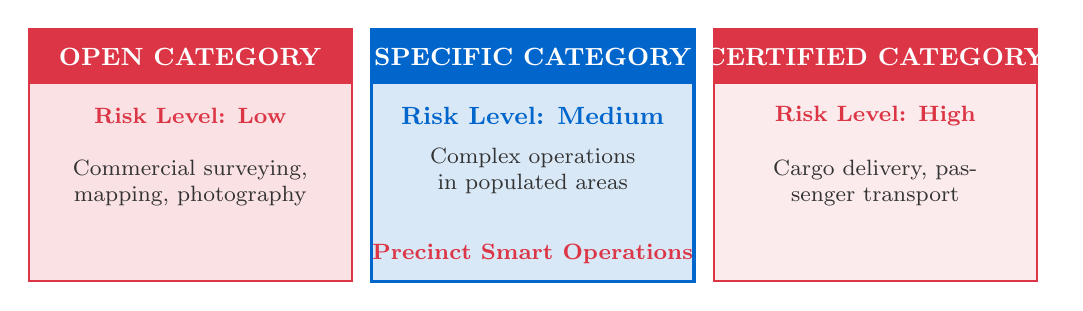
\begin{tikzpicture}[x=1cm,y=1cm]
        % Open Category card
        \fill[AccentGreen!15] (0,0) rectangle (4.1,3.2);
        \draw[AccentGreen,thick] (0,0) rectangle (4.1,3.2);
        \fill[AccentGreen] (0,2.5) rectangle (4.1,3.2);
        \node[text=white,font=\bfseries\small,align=center] at (2.05,2.85) {OPEN CATEGORY};
        \node[font=\bfseries\footnotesize,text=AccentGreen] at (2.05,2.1) {Risk Level: Low};
        \node[font=\footnotesize,text=DarkGrey,text width=3.8cm,align=center]
            at (2.05,1.25) {Commercial surveying, mapping, photography};
        % Specific Category card (highlighted — this is Precinct Smart's category)
        \fill[SecondaryBlue!15] (4.35,0) rectangle (8.45,3.2);
        \draw[SecondaryBlue,very thick] (4.35,0) rectangle (8.45,3.2);
        \fill[SecondaryBlue] (4.35,2.5) rectangle (8.45,3.2);
        \node[text=white,font=\bfseries\small,align=center] at (6.4,2.85) {SPECIFIC CATEGORY};
        \node[font=\bfseries\small,text=SecondaryBlue] at (6.4,2.1) {Risk Level: Medium};
        \node[font=\footnotesize,text=DarkGrey,text width=3.8cm,align=center]
            at (6.4,1.4) {Complex operations in populated areas};
        \node[font=\bfseries\footnotesize,text=AccentGreen,align=center]
            at (6.4,0.35) {Precinct Smart Operations};
        % Certified Category card
        \fill[AccentRed!10] (8.7,0) rectangle (12.8,3.2);
        \draw[AccentRed,thick] (8.7,0) rectangle (12.8,3.2);
        \fill[AccentRed] (8.7,2.5) rectangle (12.8,3.2);
        \node[text=white,font=\bfseries\small,align=center] at (10.75,2.85) {CERTIFIED CATEGORY};
        \node[font=\bfseries\footnotesize,text=AccentRed] at (10.75,2.1) {Risk Level: High};
        \node[font=\footnotesize,text=DarkGrey,text width=3.8cm,align=center]
            at (10.75,1.25) {Cargo delivery, passenger transport};
    \end{tikzpicture}
    \caption{CAAB Operational Categories}
    \label{tab:operational_categories}
\end{figure}

The proposed operations fall under the \textbf{Specific Category} (surveying, mapping in various areas).

\subsection{5. Insurance Requirements}

\textbf{Mandatory Insurance for All Commercial Drones:}
\begin{itemize}
    \item \textbf{Minimum Coverage:} BDT 50-100 lakhs liability insurance
    \item \textbf{Coverage Types:}
    \begin{itemize}
        \item Third-party injury or death
        \item Property damage to ground assets
        \item Equipment damage/loss during operations
    \end{itemize}
    \item \textbf{Insurance Provider:} From CAAB-approved insurers
    \item \textbf{Documentation:} Certificate must accompany all flight requests
\end{itemize}

\subsection{Land \& Geospatial Data Regulations}

\begin{itemize}
    \item \textbf{Survey of Bangladesh Coordination:} Notify and coordinate with government surveying authority
    \item \textbf{Data Classification:} Avoid military and sensitive infrastructure areas
    \item \textbf{Data Sharing Restrictions:} Government approval needed for certain data uses
    \item \textbf{Map Scale Approvals:} Large-scale maps (1:5000 or larger) may require approvals
\end{itemize}

\subsection{Business Registration \& Taxes}

\begin{itemize}
    \item Company registration with Registrar of Joint Stock Companies (RJSC)
    \item Tax Identification Number (TIN) from National Board of Revenue
    \item Import permits and custom clearance for equipment
    \item Import duty and taxes on drone and sensor equipment
\end{itemize}

\subsection{Data Protection Regulations}

\begin{itemize}
    \item Personal data handling (if applicable)
    \item Data security standards and encryption
    \item Client data confidentiality agreements
    \item Storage location restrictions (data residency)
\end{itemize}

\subsection{Regulatory Timeline \& Budget}

\textbf{Critical Path for CAAB Compliance:}

% Regulatory Timeline — TikZ flowchart with phases
\begin{figure}[H]
    \centering
    \begin{tikzpicture}[x=1cm,y=0.80cm]
        % Phase header rows and data
        % Month 0 — Business setup
        \fill[PrimaryBlue!80] (0,0) rectangle (13.0,0.80);
        \node[text=white,font=\bfseries\small,anchor=west] at (0.2,0.40)
            {Month 0 (Pre-Launch)};

        % Row 1
        \fill[LightGrey!70] (0,-0.80) rectangle (13.0,0);
        \draw[MidGrey!50] (0,-0.80) -- (13.0,-0.80);
        \node[anchor=west,font=\small,text=DarkGrey] at (0.2,-0.40)
            {Business registration (RJSC)};
        \node[anchor=west,font=\small,text=DarkGrey] at (6.0,-0.40) {Week 1--2};
        \node[anchor=west,font=\small,text=AccentGreen] at (9.5,-0.40) {BDT 1--2 lakhs};

        % Row 2
        \fill[white] (0,-1.60) rectangle (13.0,-0.80);
        \draw[MidGrey!50] (0,-1.60) -- (13.0,-1.60);
        \node[anchor=west,font=\small,text=DarkGrey] at (0.2,-1.20)
            {TIN and tax compliance (NBR)};
        \node[anchor=west,font=\small,text=DarkGrey] at (6.0,-1.20) {Week 2--3};
        \node[anchor=west,font=\small,text=AccentGreen] at (9.5,-1.20) {BDT 50K--1L};

        % Month 1-2 — Pilot Cert
        \fill[SecondaryBlue!70] (0,-2.40) rectangle (13.0,-1.60);
        \node[text=white,font=\bfseries\small,anchor=west] at (0.2,-2.00)
            {Month 1--2 (Pilot Certification)};

        % Row 3
        \fill[LightGrey!70] (0,-3.20) rectangle (13.0,-2.40);
        \draw[MidGrey!50] (0,-3.20) -- (13.0,-3.20);
        \node[anchor=west,font=\small,text=DarkGrey,text width=5.5cm] at (0.2,-2.80)
            {Avion Aerospace Academy Training (50+ hrs)};
        \node[anchor=west,font=\small,text=DarkGrey] at (6.0,-2.80) {4--6 weeks};
        \node[anchor=west,font=\small,text=AccentGreen] at (9.5,-2.80) {BDT 4--6 lakhs};

        % Row 4
        \fill[white] (0,-4.00) rectangle (13.0,-3.20);
        \draw[MidGrey!50] (0,-4.00) -- (13.0,-4.00);
        \node[anchor=west,font=\small,text=DarkGrey] at (0.2,-3.60)
            {CAAB Medical Certification (Class 3)};
        \node[anchor=west,font=\small,text=DarkGrey] at (6.0,-3.60) {Week 1--2};
        \node[anchor=west,font=\small,text=AccentGreen] at (9.5,-3.60) {BDT 50K--1L};

        % Row 5
        \fill[LightGrey!70] (0,-4.80) rectangle (13.0,-4.00);
        \draw[MidGrey!50] (0,-4.80) -- (13.0,-4.80);
        \node[anchor=west,font=\small,text=DarkGrey] at (0.2,-4.40)
            {CAAB Pilot Examination \& ROC};
        \node[anchor=west,font=\small,text=DarkGrey] at (6.0,-4.40) {Week 6--8};
        \node[anchor=west,font=\small,text=AccentGreen] at (9.5,-4.40) {BDT 1--2 lakhs};

        % Month 1-3 — Equipment
        \fill[AccentGreen!60] (0,-5.60) rectangle (13.0,-4.80);
        \node[text=white,font=\bfseries\small,anchor=west] at (0.2,-5.20)
            {Month 1--3 (Drone \& Equipment)};

        % Row 6
        \fill[white] (0,-6.40) rectangle (13.0,-5.60);
        \draw[MidGrey!50] (0,-6.40) -- (13.0,-6.40);
        \node[anchor=west,font=\small,text=DarkGrey] at (0.2,-6.00)
            {Drone equipment procurement};
        \node[anchor=west,font=\small,text=DarkGrey] at (6.0,-6.00) {Week 1--4};
        \node[anchor=west,font=\small,text=AccentGreen] at (9.5,-6.00) {BDT 80--90 lakhs};

        % Row 7
        \fill[LightGrey!70] (0,-7.20) rectangle (13.0,-6.40);
        \draw[MidGrey!50] (0,-7.20) -- (13.0,-7.20);
        \node[anchor=west,font=\small,text=DarkGrey] at (0.2,-6.80)
            {CAAB Drone Registration (online)};
        \node[anchor=west,font=\small,text=DarkGrey] at (6.0,-6.80) {Week 8--12};
        \node[anchor=west,font=\small,text=AccentGreen] at (9.5,-6.80) {BDT 50K--1L};

        % Row 8
        \fill[white] (0,-8.00) rectangle (13.0,-7.20);
        \draw[MidGrey!50] (0,-8.00) -- (13.0,-8.00);
        \node[anchor=west,font=\small,text=DarkGrey] at (0.2,-7.60)
            {Equipment import permits \& customs};
        \node[anchor=west,font=\small,text=DarkGrey] at (6.0,-7.60) {Month 1--2};
        \node[anchor=west,font=\small,text=AccentGreen] at (9.5,-7.60) {BDT 2--3 lakhs};

        % Row 9 — Insurance
        \fill[LightGrey!70] (0,-8.80) rectangle (13.0,-8.00);
        \draw[MidGrey!50] (0,-8.80) -- (13.0,-8.80);
        \node[anchor=west,font=\small,text=DarkGrey] at (0.2,-8.40)
            {Insurance (3-year liability coverage)};
        \node[anchor=west,font=\small,text=DarkGrey] at (6.0,-8.40) {Month 1};
        \node[anchor=west,font=\small,text=AccentGreen] at (9.5,-8.40) {BDT 10--15 lakhs};

        % Total rows
        \fill[PrimaryBlue!12] (0,-9.60) rectangle (13.0,-8.80);
        \draw[PrimaryBlue] (0,-9.60) rectangle (13.0,-8.80);
        \node[anchor=west,font=\small\bfseries,text=PrimaryBlue] at (0.2,-9.20)
            {TOTAL (Pre-Launch)};
        \node[anchor=west,font=\small\bfseries,text=AccentGreen] at (9.5,-9.20) {BDT 21--35 lakhs};

        \fill[PrimaryBlue!20] (0,-10.40) rectangle (13.0,-9.60);
        \draw[PrimaryBlue,thick] (0,-10.40) rectangle (13.0,-9.60);
        \node[anchor=west,font=\small\bfseries,text=PrimaryBlue] at (0.2,-10.00)
            {TOTAL (First Year, incl.\ operations)};
        \node[anchor=west,font=\small\bfseries,text=AccentGreen] at (9.5,-10.00) {BDT 25--45 lakhs};

        % Outer border + column lines
        \draw[PrimaryBlue,thick] (0,-10.40) rectangle (13.0,0.80);
        \foreach \xd in {5.95,9.45}{
            \draw[MidGrey!70] (\xd,-10.40) -- (\xd,0.80);
        }
        % Column headers
        \node[text=white,font=\bfseries\small,anchor=west] at (6.1,0.40) {Timeline};
        \node[text=white,font=\bfseries\small,anchor=west] at (9.6,0.40) {Est. Cost (BDT)};
    \end{tikzpicture}
    \caption{Regulatory Compliance Timeline \& Costs (CAAB-Based)}
    \label{tab:regulatory_timeline}
\end{figure}

\textbf{Key Timeline Notes:}
\begin{itemize}
    \item \textbf{Pilot Certification:} Can be done in parallel (4-6 weeks via Avion Aerospace)
    \item \textbf{Drone Registration:} Must be completed BEFORE operations
    \item \textbf{Flight Approvals:} Require 45-day advance submission to CAAB
    \item \textbf{Critical Path:} Pilot training + Drone registration = 6-8 weeks minimum
    \item \textbf{First Flight:} Possible Month 3 (after all approvals)
    \item \textbf{Regular Operations:} All flights need 45-day FSR advance notice
\end{itemize}

\textbf{Updated Equipment Investment (includes regulatory costs):}

Total startup capex increases from BDT 90.6L to approximately BDT 100-110L when including regulatory compliance, training, insurance, and import permits. This fits within the planned BDT 100-125L initial investment.

\section{Operational Workflow}

\subsection{Project Execution Flow}

\begin{enumerate}
    \item \textbf{Project Scoping (Week 1)}
        \begin{itemize}
            \item Client requirements assessment
            \item Area survey and flight planning
            \item Regulatory approvals (CAAB flight path)
            \item Resource allocation
        \end{itemize}

    \item \textbf{Data Collection (Week 2-3)}
        \begin{itemize}
            \item Ground control points (GCP) establishment
            \item Drone flights (weather dependent)
            \item Data quality assurance
            \item Backup data creation
        \end{itemize}

    \item \textbf{Processing (Week 4-6)}
        \begin{itemize}
            \item LiDAR point cloud processing
            \item Photogrammetry alignment and meshing
            \item Accuracy verification and calibration
            \item Analysis and interpretation
        \end{itemize}

    \item \textbf{Delivery \& Support (Week 7-8)}
        \begin{itemize}
            \item Report and map generation
            \item Client presentation and Q\&A
            \item Data delivery (cloud or physical)
            \item Post-delivery support
        \end{itemize}
\end{enumerate}

% ============================================================================
% END OF CHAPTER 3
% ============================================================================


% Chapter 4: Financial Projections
% ============================================================================
% CHAPTER 4: FINANCIAL PROJECTIONS
% ============================================================================

\chapter{Financial Projections}

\section{Initial Investment Breakdown}

The total startup capital required is shown in the following detailed breakdown:

% Startup Capital — pgf-pie chart
\begin{figure}[H]
    \centering
    \begin{tikzpicture}
        \pie[
            radius=3.0,
            color={SecondaryBlue!80, AccentGreen!70, AccentOrange!80, AccentRed!60, MidGrey!80},
            text=legend,
            style={drop shadow},
            before number=\phantom{},
            after number=\%,
            sum=100
        ]{
            68/Equipment \& Hardware (68\%),
            4/Office Setup (4\%),
            5/Software Licenses (5\%),
            11/Regulatory \& Compliance (11\%),
            12/Working Capital (12\%)
        }
    \end{tikzpicture}
    \caption{Total Startup Capital Requirement (BDT 132.6 Lakhs)}
    \label{tab:startup_capital}
\end{figure}

\noindent
\begin{minipage}[t]{0.48\textwidth}
    \begin{tcolorbox}[colback=BoxBlue,colframe=SecondaryBlue,arc=4pt,boxrule=1pt,
        top=6pt,bottom=6pt,left=8pt,right=8pt]
        \small
        \textbf{\textcolor{PrimaryBlue}{Capital Breakdown:}}\\[4pt]
        \textbf{Equipment \& Hardware:} BDT 90.6L (68\%)\\
        \textbf{Office Setup:} BDT 5L (4\%)\\
        \textbf{Software Licenses:} BDT 7L (5\%)\\
        \textbf{Regulatory \& Compliance:} BDT 15L (11\%)\\
        \textbf{Working Capital:} BDT 15L (12\%)
    \end{tcolorbox}
\end{minipage}\hfill
\begin{minipage}[t]{0.48\textwidth}
    \begin{tcolorbox}[colback=BoxGreen,colframe=AccentGreen,arc=4pt,boxrule=1pt,
        top=6pt,bottom=6pt,left=8pt,right=8pt,halign=center]
        {\large\bfseries\color{AccentGreen}BDT 132.6 Lakhs}\\[4pt]
        {\small\color{DarkGrey}Total Capital Required}\\[2pt]
        {\small\color{DarkGrey}Recommendation: BDT 100--125L minimum\\
        (132.6L provides optimal cushion)}
    \end{tcolorbox}
\end{minipage}

\section{Year-by-Year Revenue Projections}

\subsection{YEAR 1: Foundation \& Market Entry}

\textbf{Operational Target:} 5-8 projects, 12-15 sq. km coverage

% Year 1 Revenue — pgfplots bar chart
\begin{figure}[H]
    \centering
    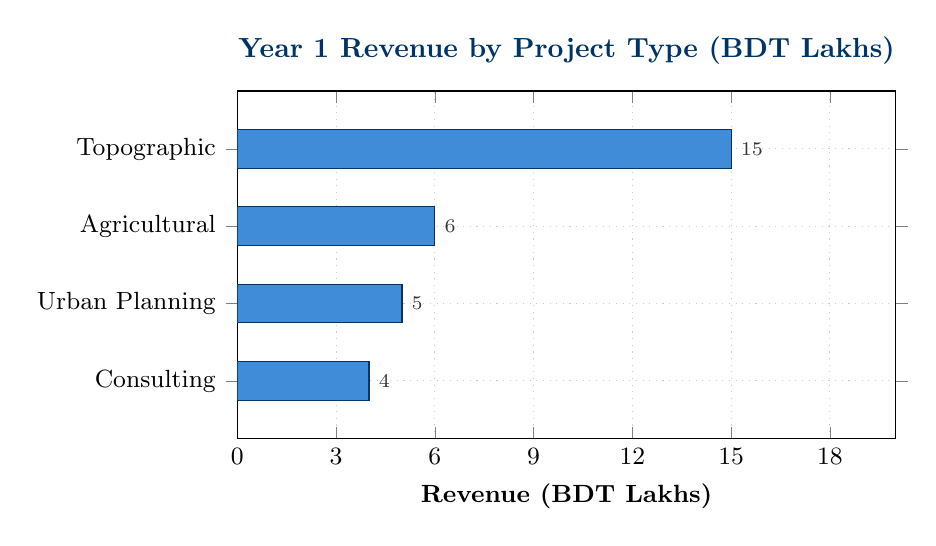
\begin{tikzpicture}
        \begin{axis}[
            xbar,
            bar width=14pt,
            width=0.82\textwidth,
            height=6cm,
            enlarge y limits=0.25,
            symbolic y coords={Consulting,Urban Planning,Agricultural,Topographic},
            ytick=data,
            xlabel={\textbf{Revenue (BDT Lakhs)}},
            xmin=0, xmax=20,
            xtick={0,3,6,9,12,15,18},
            grid=major,
            grid style={dotted,gray!40},
            title={\textbf{Year 1 Revenue by Project Type (BDT Lakhs)}},
            title style={font=\normalsize\bfseries\color{PrimaryBlue}},
            tick label style={font=\small},
            label style={font=\small\bfseries},
            nodes near coords,
            nodes near coords style={font=\scriptsize\bfseries,color=DarkGrey},
        ]
        \addplot[fill=SecondaryBlue!75,draw=PrimaryBlue] coordinates {
            (4,Consulting)(5,Urban Planning)(6,Agricultural)(15,Topographic)
        };
        \end{axis}
    \end{tikzpicture}
    \caption{Year 1 Revenue Projection (Conservative Scenario)}
    \label{tab:year1_revenue}
\end{figure}

% Year 1 Operating Costs — tcolorbox KPI grid
\begin{figure}[H]
    \centering
    \noindent
    \begin{minipage}[t]{0.32\textwidth}
        \begin{tcolorbox}[colback=BoxBlue,colframe=SecondaryBlue,arc=5pt,boxrule=1pt,
            halign=center,top=6pt,bottom=6pt]
            {\large\bfseries\color{PrimaryBlue}BDT 18L}\\[2pt]
            {\small\color{DarkGrey}Staff Salaries\\(12 people)}
        \end{tcolorbox}
    \end{minipage}\hfill
    \begin{minipage}[t]{0.32\textwidth}
        \begin{tcolorbox}[colback=BoxBlue,colframe=SecondaryBlue,arc=5pt,boxrule=1pt,
            halign=center,top=6pt,bottom=6pt]
            {\large\bfseries\color{PrimaryBlue}BDT 5L}\\[2pt]
            {\small\color{DarkGrey}Office + Equipment\\Maintenance}
        \end{tcolorbox}
    \end{minipage}\hfill
    \begin{minipage}[t]{0.32\textwidth}
        \begin{tcolorbox}[colback=BoxBlue,colframe=SecondaryBlue,arc=5pt,boxrule=1pt,
            halign=center,top=6pt,bottom=6pt]
            {\large\bfseries\color{PrimaryBlue}BDT 5L}\\[2pt]
            {\small\color{DarkGrey}Travel + Marketing\\+ Misc.}
        \end{tcolorbox}
    \end{minipage}
    \caption{Year 1 Operating Costs (Total: BDT 28 Lakhs)}
    \label{tab:year1_costs}
\end{figure}

\textbf{Year 1 Financial Summary:}
\begin{itemize}
    \item Total Revenue: BDT 30 lakhs
    \item Operating Costs: BDT 28 lakhs
    \item \textcolor{AccentGreen}{\textbf{Net Profit/Loss: +2 lakhs}} (Break-even achieved)
    \item Break-even Timeline: \textcolor{AccentGreen}{\textbf{Month 10}}
\end{itemize}

\subsection{YEAR 2: Growth \& Expansion}

\textbf{Operational Target:} 15-20 projects, 30-40 sq. km coverage, 2 hubs operational

% Year 2 Revenue — pgfplots bar chart
\begin{figure}[H]
    \centering
    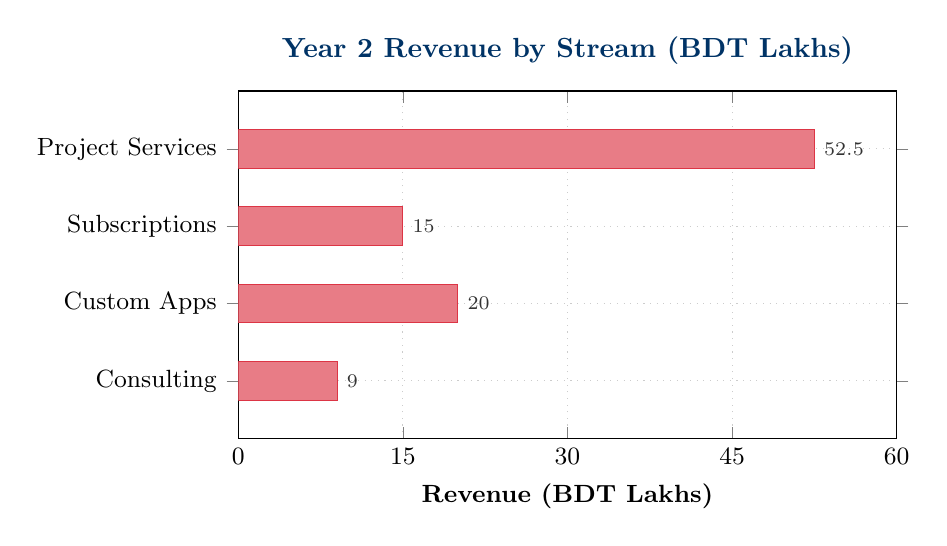
\begin{tikzpicture}
        \begin{axis}[
            xbar,
            bar width=14pt,
            width=0.82\textwidth,
            height=6cm,
            enlarge y limits=0.25,
            symbolic y coords={Consulting,Custom Apps,Subscriptions,Project Services},
            ytick=data,
            xlabel={\textbf{Revenue (BDT Lakhs)}},
            xmin=0, xmax=60,
            xtick={0,15,30,45,60},
            grid=major,
            grid style={dotted,gray!40},
            title={\textbf{Year 2 Revenue by Stream (BDT Lakhs)}},
            title style={font=\normalsize\bfseries\color{PrimaryBlue}},
            tick label style={font=\small},
            label style={font=\small\bfseries},
            nodes near coords,
            nodes near coords style={font=\scriptsize\bfseries,color=DarkGrey},
        ]
        \addplot[fill=AccentGreen!65,draw=AccentGreen] coordinates {
            (9,Consulting)(20,Custom Apps)(15,Subscriptions)(52.5,Project Services)
        };
        \end{axis}
    \end{tikzpicture}
    \caption{Year 2 Revenue Projection (Growth Scenario)}
    \label{tab:year2_revenue}
\end{figure}

% Year 2 Operating Costs — tcolorbox KPI grid
\begin{figure}[H]
    \centering
    \noindent
    \begin{minipage}[t]{0.32\textwidth}
        \begin{tcolorbox}[colback=BoxBlue,colframe=SecondaryBlue,arc=5pt,boxrule=1pt,
            halign=center,top=6pt,bottom=6pt]
            {\large\bfseries\color{PrimaryBlue}BDT 28L}\\[2pt]
            {\small\color{DarkGrey}Staff Salaries\\(18 people)}
        \end{tcolorbox}
    \end{minipage}\hfill
    \begin{minipage}[t]{0.32\textwidth}
        \begin{tcolorbox}[colback=BoxBlue,colframe=SecondaryBlue,arc=5pt,boxrule=1pt,
            halign=center,top=6pt,bottom=6pt]
            {\large\bfseries\color{PrimaryBlue}BDT 10L}\\[2pt]
            {\small\color{DarkGrey}Office + 2 Hubs\\Equipment}
        \end{tcolorbox}
    \end{minipage}\hfill
    \begin{minipage}[t]{0.32\textwidth}
        \begin{tcolorbox}[colback=BoxBlue,colframe=SecondaryBlue,arc=5pt,boxrule=1pt,
            halign=center,top=6pt,bottom=6pt]
            {\large\bfseries\color{PrimaryBlue}BDT 9L}\\[2pt]
            {\small\color{DarkGrey}Travel + Marketing\\+ Misc.}
        \end{tcolorbox}
    \end{minipage}
    \caption{Year 2 Operating Costs (Total: BDT 47 Lakhs)}
    \label{tab:year2_costs}
\end{figure}

\textbf{Year 2 Financial Summary:}
\begin{itemize}
    \item Total Revenue: BDT 96.5 lakhs
    \item Operating Costs: BDT 47 lakhs
    \item \textcolor{AccentGreen}{\textbf{Net Profit: 49.5 lakhs}}
    \item Profit Margin: 51\%
    \item Cumulative Profit (Y1+Y2): BDT 51.5 lakhs
\end{itemize}

\subsection{YEAR 3: Scaling \& Consolidation}

\textbf{Operational Target:} 40-50 projects, 70-80 sq. km coverage, 3+ hubs, Data Science platform scaling

% Year 3 Revenue — pgfplots bar chart
\begin{figure}[H]
    \centering
    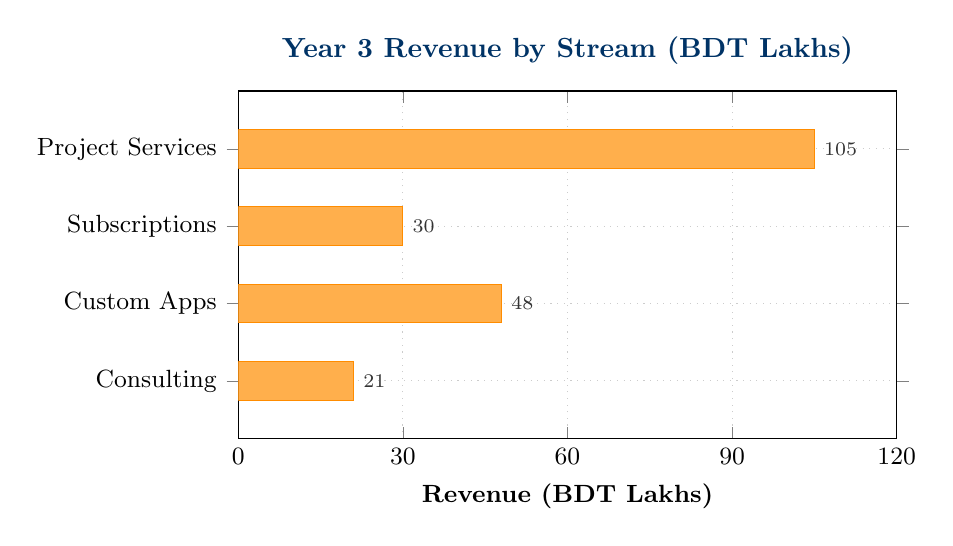
\begin{tikzpicture}
        \begin{axis}[
            xbar,
            bar width=14pt,
            width=0.82\textwidth,
            height=6cm,
            enlarge y limits=0.25,
            symbolic y coords={Consulting,Custom Apps,Subscriptions,Project Services},
            ytick=data,
            xlabel={\textbf{Revenue (BDT Lakhs)}},
            xmin=0, xmax=120,
            xtick={0,30,60,90,120},
            grid=major,
            grid style={dotted,gray!40},
            title={\textbf{Year 3 Revenue by Stream (BDT Lakhs)}},
            title style={font=\normalsize\bfseries\color{PrimaryBlue}},
            tick label style={font=\small},
            label style={font=\small\bfseries},
            nodes near coords,
            nodes near coords style={font=\scriptsize\bfseries,color=DarkGrey},
        ]
        \addplot[fill=AccentOrange!70,draw=AccentOrange] coordinates {
            (21,Consulting)(48,Custom Apps)(30,Subscriptions)(105,Project Services)
        };
        \end{axis}
    \end{tikzpicture}
    \caption{Year 3 Revenue Projection (Scaling Scenario)}
    \label{tab:year3_revenue}
\end{figure}

% Year 3 Operating Costs — tcolorbox KPI grid
\begin{figure}[H]
    \centering
    \noindent
    \begin{minipage}[t]{0.32\textwidth}
        \begin{tcolorbox}[colback=BoxBlue,colframe=SecondaryBlue,arc=5pt,boxrule=1pt,
            halign=center,top=6pt,bottom=6pt]
            {\large\bfseries\color{PrimaryBlue}BDT 40L}\\[2pt]
            {\small\color{DarkGrey}Staff Salaries\\(22--25 people)}
        \end{tcolorbox}
    \end{minipage}\hfill
    \begin{minipage}[t]{0.32\textwidth}
        \begin{tcolorbox}[colback=BoxBlue,colframe=SecondaryBlue,arc=5pt,boxrule=1pt,
            halign=center,top=6pt,bottom=6pt]
            {\large\bfseries\color{PrimaryBlue}BDT 16L}\\[2pt]
            {\small\color{DarkGrey}Office (3--4 Hubs)\\R\&D + Equipment}
        \end{tcolorbox}
    \end{minipage}\hfill
    \begin{minipage}[t]{0.32\textwidth}
        \begin{tcolorbox}[colback=BoxBlue,colframe=SecondaryBlue,arc=5pt,boxrule=1pt,
            halign=center,top=6pt,bottom=6pt]
            {\large\bfseries\color{PrimaryBlue}BDT 12L}\\[2pt]
            {\small\color{DarkGrey}Travel + Marketing\\+ Misc.}
        \end{tcolorbox}
    \end{minipage}
    \caption{Year 3 Operating Costs (Total: BDT 68 Lakhs)}
    \label{tab:year3_costs}
\end{figure}

\textbf{Year 3 Financial Summary:}
\begin{itemize}
    \item Total Revenue: BDT 204 lakhs
    \item Operating Costs: BDT 68 lakhs
    \item \textcolor{AccentGreen}{\textbf{Net Profit: 136 lakhs}}
    \item Profit Margin: 67\%
    \item Cumulative Profit (Y1+Y2+Y3): BDT 187.5 lakhs
\end{itemize}

\section{3-Year Summary \& Key Metrics}

% 3-Year Summary — grouped bar chart
\begin{figure}[H]
    \centering
    \begin{tikzpicture}
        \begin{axis}[
            ybar,
            bar width=18pt,
            width=0.92\textwidth,
            height=7cm,
            enlarge x limits=0.25,
            symbolic x coords={Year 1, Year 2, Year 3},
            xtick=data,
            xlabel={\textbf{Year}},
            ylabel={\textbf{BDT (Lakhs)}},
            ymin=0, ymax=230,
            ytick={0,50,100,150,200},
            grid=major,
            grid style={dotted, gray!40},
            legend style={at={(0.98,0.97)}, anchor=north east,
                          font=\small, draw=MidGrey, fill=LightGrey},
            tick label style={font=\small},
            label style={font=\small\bfseries},
            title={\textbf{3-Year Financial Overview (BDT Lakhs)}},
            title style={font=\normalsize\bfseries\color{PrimaryBlue}},
            axis line style={color=DarkGrey},
            nodes near coords,
            nodes near coords style={font=\scriptsize\bfseries, color=DarkGrey},
            every node near coord/.append style={rotate=0, anchor=south},
        ]
        % Revenue bars
        \addplot[fill=SecondaryBlue!80, draw=PrimaryBlue] coordinates {
            (Year 1, 30) (Year 2, 96.5) (Year 3, 204)
        };
        % Cost bars
        \addplot[fill=AccentRed!60, draw=AccentRed] coordinates {
            (Year 1, 28) (Year 2, 47) (Year 3, 68)
        };
        % Profit bars
        \addplot[fill=AccentGreen!70, draw=AccentGreen] coordinates {
            (Year 1, 2) (Year 2, 49.5) (Year 3, 136)
        };
        \legend{Revenue, Operating Costs, Net Profit}
        \end{axis}
    \end{tikzpicture}
    \caption{3-Year Revenue, Cost, and Profit Overview}
    \label{fig:revenue_growth}
\end{figure}

% 3-Year Summary KPI cards
\begin{figure}[H]
    \centering
    \begin{tikzpicture}[x=1cm,y=0.82cm]
        % Header
        \fill[PrimaryBlue] (0,0) rectangle (13.5,0.82);
        \foreach \xpos/\lbl in {
            0.1/{Metric},
            3.4/{Year 1},
            6.0/{Year 2},
            8.9/{Year 3}}{
            \node[text=white,font=\bfseries\small,anchor=west] at (\xpos,0.41) {\lbl};
        }
        % Summary rows
        \foreach \row/\metric/\ya/\yb/\yc in {
            1/{Revenue (BDT Lakhs)}/{30}/{96.5}/{204},
            2/{Operating Costs}/{28}/{47}/{68},
            3/{Net Profit}/{2}/{49.5}/{136},
            4/{Profit Margin}/{7\%}/{51\%}/{67\%},
            5/{Break-even Month}/{10}/{2 (at start)}/{--},
            6/{ROI}/{1.5\%}/{49\%}/{104\%},
            7/{Payback Period}/{45 mo.}/{24 mo.}/{11 mo.}
        }{
            \pgfmathsetmacro{\ybot}{-(\row-1)*0.82}
            \pgfmathsetmacro{\ytop}{\ybot+0.82}
            \ifodd\row
                \fill[LightGrey!60] (0,\ybot) rectangle (13.5,\ytop);
            \fi
            \draw[MidGrey!50] (0,\ybot) -- (13.5,\ybot);
            \node[anchor=west,font=\small\bfseries,text=PrimaryBlue] at (0.1,\ybot+0.41) {\metric};
            \node[anchor=west,font=\small,text=DarkGrey] at (3.4,\ybot+0.41) {\ya};
            \node[anchor=west,font=\small\bfseries,text=SecondaryBlue] at (6.0,\ybot+0.41) {\yb};
            \node[anchor=west,font=\small\bfseries,text=AccentGreen] at (8.9,\ybot+0.41) {\yc};
        }
        % Cumulative profit row
        \fill[AccentGreen!15] (0,-5.74) rectangle (13.5,-4.92);
        \draw[AccentGreen,thick] (0,-5.74) rectangle (13.5,-4.92);
        \node[anchor=west,font=\small\bfseries,text=PrimaryBlue] at (0.1,-5.33) {Cumulative Profit};
        \node[anchor=west,font=\small\bfseries,text=DarkGrey] at (3.4,-5.33) {BDT 2L};
        \node[anchor=west,font=\small\bfseries,text=SecondaryBlue] at (6.0,-5.33) {BDT 51.5L};
        \node[anchor=west,font=\small\bfseries,text=AccentGreen] at (8.9,-5.33) {BDT 187.5L};
        % Outer border + column lines
        \draw[PrimaryBlue,thick] (0,-5.74) rectangle (13.5,0.82);
        \foreach \xd in {3.35,5.95,8.85}{
            \draw[MidGrey!70] (\xd,-5.74) -- (\xd,0.82);
        }
    \end{tikzpicture}
    \caption{3-Year Financial Summary}
    \label{tab:3year_summary}
\end{figure}

\begin{successbox}[3-Year Financial Highlights]
    \begin{tabular}{@{}llll@{}}
        \textbf{Metric} & \textbf{Year 1} & \textbf{Year 2} & \textbf{Year 3} \\
        Revenue growth  & BDT 30L         & +222\%          & +111\%          \\
        Profit margin   & 7\%             & 51\%            & 67\%            \\
        Cumulative profit & BDT 2L        & BDT 51.5L       & BDT 187.5L      \\
    \end{tabular}
\end{successbox}

\section{Cost Structure per Service}

Understanding the actual cost to deliver each service is critical for pricing and margin management:

\subsection{Topographic Survey Project (500 hectares)}

\textbf{Service Overview:} High-resolution LiDAR-based topographic mapping for infrastructure planning, flood risk assessment, and land management. A 500-hectare survey produces a Digital Elevation Model (DEM), Digital Terrain Model (DTM), and contour maps at 10--50\,cm accuracy.

\textbf{Typical Clients:} Government land agencies (DLRS, LGED), infrastructure developers, and environmental consultancies.

\textbf{Scope \& Timeline:}
\begin{itemize}
    \item \textbf{Pre-flight:} Ground control point (GCP) placement, flight plan approval --- 2--3 days
    \item \textbf{Data Acquisition:} 2--3 flight days covering 500 ha at 60\,m altitude
    \item \textbf{Processing:} Point cloud classification, DEM/DTM generation, QA --- 5--7 days
    \item \textbf{Deliverables:} GeoTIFF rasters, LAS point cloud, contour shapefile, PDF report
    \item \textbf{Total Project Duration:} 2--3 weeks
\end{itemize}

% Survey cost breakdown — TikZ card
\begin{figure}[H]
    \centering
    \begin{tikzpicture}[x=1cm,y=0.82cm]
        % Header
        \fill[PrimaryBlue] (0,0) rectangle (13.0,0.82);
        \foreach \xpos/\lbl in {0.1/{Cost Element}, 6.5/{Hours / Unit}, 9.5/{Amount (BDT)}}{
            \node[text=white,font=\bfseries\small,anchor=west] at (\xpos,0.41) {\lbl};
        }
        % Cost rows
        \foreach \row/\el/\hrs/\amt in {
            1/{Drone flight operations (pilot + equipment)}/{20 hrs @ 4\,000/hr}/{80\,000},
            2/{Point cloud processing \& DEM generation}/{40 hrs @ 500/hr}/{20\,000},
            3/{Equipment depreciation (LiDAR sensor)}/{Per mission}/{10\,000},
            4/{Travel, accommodation \& field logistics}/{Lump sum}/{20\,000}
        }{
            \pgfmathsetmacro{\ybot}{-(\row-1)*0.82}
            \pgfmathsetmacro{\ytop}{\ybot+0.82}
            \ifodd\row
                \fill[LightGrey!60] (0,\ybot) rectangle (13.0,\ytop);
            \fi
            \draw[MidGrey!50] (0,\ybot) -- (13.0,\ybot);
            \node[anchor=west,font=\small,text=DarkGrey,text width=6.2cm] at (0.1,\ybot+0.41) {\el};
            \node[anchor=west,font=\small,text=DarkGrey] at (6.5,\ybot+0.41) {\hrs};
            \node[anchor=west,font=\small,text=DarkGrey] at (9.5,\ybot+0.41) {\amt};
        }
        % Total delivery cost
        \fill[PrimaryBlue!15] (0,-3.28) rectangle (13.0,-2.46);
        \draw[PrimaryBlue] (0,-3.28) -- (13.0,-3.28);
        \node[anchor=west,font=\small\bfseries,text=PrimaryBlue] at (0.1,-2.87) {Total Delivery Cost};
        \node[anchor=west,font=\small\bfseries,text=PrimaryBlue] at (9.5,-2.87) {BDT 1,30,000};
        % Selling price
        \fill[AccentGreen!15] (0,-4.10) rectangle (13.0,-3.28);
        \draw[AccentGreen!60] (0,-4.10) -- (13.0,-4.10);
        \node[anchor=west,font=\small\bfseries,text=AccentGreen] at (0.1,-3.69) {Selling Price (value-based)};
        \node[anchor=west,font=\small\bfseries,text=AccentGreen] at (9.5,-3.69) {BDT 3,50,000 -- 5,00,000};
        % Margin
        \fill[AccentGreen!25] (0,-4.92) rectangle (13.0,-4.10);
        \draw[AccentGreen,thick] (0,-4.92) rectangle (13.0,-4.10);
        \node[anchor=west,font=\small\bfseries,text=AccentGreen] at (0.1,-4.51) {Gross Margin};
        \node[anchor=west,font=\small\bfseries,text=AccentGreen] at (9.5,-4.51) {62--74\%};
        % Outer border + column lines
        \draw[PrimaryBlue,thick] (0,-4.92) rectangle (13.0,0.82);
        \foreach \xd in {6.45,9.45}{
            \draw[MidGrey!70] (\xd,-4.92) -- (\xd,0.82);
        }
    \end{tikzpicture}
    \caption{Cost Breakdown: Topographic Survey (500 ha)}
    \label{tab:survey_cost}
\end{figure}

\begin{successbox}[Pricing Rationale]
    Government procurement benchmarks for equivalent survey work range from BDT\,4,00,000--8,00,000 per 500\,ha. Precinct Smart's LiDAR accuracy (vs.\ traditional total station methods) justifies a premium while remaining 30--40\% below legacy survey firm rates.
\end{successbox}

% ---

\subsection{Agricultural Mapping (1,000 hectares)}

\textbf{Service Overview:} Multispectral and LiDAR drone mapping of agricultural land to generate crop health indices (NDVI, NDRE), soil variability maps, and drainage models. Delivered to NGO partners, agricultural departments, and commercial farms.

\textbf{Typical Clients:} BRAC, DAE (Department of Agricultural Extension), large commercial farms, and irrigation boards.

\textbf{Scope \& Timeline:}
\begin{itemize}
    \item \textbf{Pre-flight:} Crop calendar coordination, sensor calibration, GCP setup --- 1--2 days
    \item \textbf{Data Acquisition:} 3--4 flight days covering 1,000\,ha with multispectral payload
    \item \textbf{Processing:} Orthomosaic, NDVI raster, zone management maps --- 5--6 days
    \item \textbf{Deliverables:} Prescription maps, NDVI time-series, agronomist report, field-ready PDF
    \item \textbf{Total Project Duration:} 2--3 weeks
\end{itemize}

% Agricultural mapping cost — TikZ card
\begin{figure}[H]
    \centering
    \begin{tikzpicture}[x=1cm,y=0.82cm]
        % Header
        \fill[AccentGreen!70] (0,0) rectangle (13.0,0.82);
        \foreach \xpos/\lbl in {0.1/{Cost Element}, 6.5/{Hours / Unit}, 9.5/{Amount (BDT)}}{
            \node[text=white,font=\bfseries\small,anchor=west] at (\xpos,0.41) {\lbl};
        }
        % Cost rows
        \foreach \row/\el/\hrs/\amt in {
            1/{Drone flight operations (multispectral)}/{35 hrs}/{1,40,000},
            2/{Spectral processing \& index generation}/{25 hrs @ 500/hr}/{12,500},
            3/{Travel \& field accommodation}/{Lump sum}/{40,000},
            4/{Equipment \& sensor consumables}/{Per mission}/{20,000}
        }{
            \pgfmathsetmacro{\ybot}{-(\row-1)*0.82}
            \pgfmathsetmacro{\ytop}{\ybot+0.82}
            \ifodd\row
                \fill[LightGrey!60] (0,\ybot) rectangle (13.0,\ytop);
            \fi
            \draw[MidGrey!50] (0,\ybot) -- (13.0,\ybot);
            \node[anchor=west,font=\small,text=DarkGrey,text width=6.2cm] at (0.1,\ybot+0.41) {\el};
            \node[anchor=west,font=\small,text=DarkGrey] at (6.5,\ybot+0.41) {\hrs};
            \node[anchor=west,font=\small,text=DarkGrey] at (9.5,\ybot+0.41) {\amt};
        }
        % Total delivery cost
        \fill[AccentGreen!15] (0,-3.28) rectangle (13.0,-2.46);
        \draw[AccentGreen] (0,-3.28) -- (13.0,-3.28);
        \node[anchor=west,font=\small\bfseries,text=AccentGreen] at (0.1,-2.87) {Total Delivery Cost};
        \node[anchor=west,font=\small\bfseries,text=AccentGreen] at (9.5,-2.87) {BDT 2,12,500};
        % Selling price
        \fill[AccentGreen!25] (0,-4.10) rectangle (13.0,-3.28);
        \draw[AccentGreen!60] (0,-4.10) -- (13.0,-4.10);
        \node[anchor=west,font=\small\bfseries,text=AccentGreen] at (0.1,-3.69) {Selling Price (value-based)};
        \node[anchor=west,font=\small\bfseries,text=AccentGreen] at (9.5,-3.69) {BDT 4,00,000 -- 6,00,000};
        % Margin
        \fill[AccentGreen!35] (0,-4.92) rectangle (13.0,-4.10);
        \draw[AccentGreen,thick] (0,-4.92) rectangle (13.0,-4.10);
        \node[anchor=west,font=\small\bfseries,text=AccentGreen] at (0.1,-4.51) {Gross Margin};
        \node[anchor=west,font=\small\bfseries,text=AccentGreen] at (9.5,-4.51) {50--65\%};
        % Outer border + column lines
        \draw[AccentGreen!80,thick] (0,-4.92) rectangle (13.0,0.82);
        \foreach \xd in {6.45,9.45}{
            \draw[MidGrey!70] (\xd,-4.92) -- (\xd,0.82);
        }
    \end{tikzpicture}
    \caption{Cost Breakdown: Agricultural Mapping (1,000 ha)}
    \label{tab:agri_cost}
\end{figure}

\begin{successbox}[Farmer ROI Justification]
    A 1,000\,ha precision agriculture map enables yield gains of 5--15\% for participating farmers. At average paddy yield of BDT\,1,20,000/ha, a 10\% improvement across 1,000\,ha generates BDT\,1.2\,crore in additional farmer income --- making a BDT\,4,00,000--6,00,000 mapping fee highly cost-effective.
\end{successbox}

% ---

\subsection{Custom GIS Application}

\textbf{Service Overview:} End-to-end development of web or mobile GIS applications tailored to client workflows. Typical products include land record portals, crop monitoring dashboards, real-time flood alert systems, and farmer advisory apps integrated with drone data pipelines.

\textbf{Typical Clients:} Government ministries (MoLand, MoA), NGOs requiring digital field tools, agri-fintech companies, and real estate developers.

\textbf{Scope \& Timeline:}
\begin{itemize}
    \item \textbf{Discovery:} Requirements workshops, UX wireframes, technical architecture --- 1--2 weeks
    \item \textbf{Development:} Backend (Django/FastAPI), frontend (React), GIS layers (PostGIS/GeoServer) --- 6--10 weeks
    \item \textbf{Integration:} Drone data pipeline, satellite feed, or IoT sensor connection --- 2--3 weeks
    \item \textbf{Testing \& Deployment:} UAT, cloud deployment (AWS/GCP), user training --- 1--2 weeks
    \item \textbf{Deliverables:} Source code, documentation, hosted application, 3-month support
    \item \textbf{Total Project Duration:} 3--4 months
\end{itemize}

% Custom GIS App cost — TikZ card
\begin{figure}[H]
    \centering
    \begin{tikzpicture}[x=1cm,y=0.82cm]
        % Header
        \fill[SecondaryBlue!85] (0,0) rectangle (13.0,0.82);
        \foreach \xpos/\lbl in {0.1/{Cost Element}, 6.5/{Hours / Unit}, 9.5/{Amount (BDT)}}{
            \node[text=white,font=\bfseries\small,anchor=west] at (\xpos,0.41) {\lbl};
        }
        % Cost rows
        \foreach \row/\el/\hrs/\amt in {
            1/{Requirements, UX design \& architecture}/{60 hrs}/{30,000},
            2/{Backend \& GIS development}/{100 hrs}/{50,000},
            3/{Testing, QA \& deployment}/{40 hrs}/{20,000},
            4/{Cloud infrastructure setup (AWS/GCP)}/{Lump sum}/{50,000},
            5/{Technical documentation \& training}/{Lump sum}/{10,000}
        }{
            \pgfmathsetmacro{\ybot}{-(\row-1)*0.82}
            \pgfmathsetmacro{\ytop}{\ybot+0.82}
            \ifodd\row
                \fill[LightGrey!60] (0,\ybot) rectangle (13.0,\ytop);
            \fi
            \draw[MidGrey!50] (0,\ybot) -- (13.0,\ybot);
            \node[anchor=west,font=\small,text=DarkGrey,text width=6.2cm] at (0.1,\ybot+0.41) {\el};
            \node[anchor=west,font=\small,text=DarkGrey] at (6.5,\ybot+0.41) {\hrs};
            \node[anchor=west,font=\small,text=DarkGrey] at (9.5,\ybot+0.41) {\amt};
        }
        % Total delivery cost
        \fill[SecondaryBlue!15] (0,-4.10) rectangle (13.0,-3.28);
        \draw[SecondaryBlue] (0,-4.10) -- (13.0,-4.10);
        \node[anchor=west,font=\small\bfseries,text=PrimaryBlue] at (0.1,-3.69) {Total Delivery Cost};
        \node[anchor=west,font=\small\bfseries,text=PrimaryBlue] at (9.5,-3.69) {BDT 1,60,000};
        % Selling price
        \fill[SecondaryBlue!20] (0,-4.92) rectangle (13.0,-4.10);
        \draw[SecondaryBlue!60] (0,-4.92) -- (13.0,-4.92);
        \node[anchor=west,font=\small\bfseries,text=AccentGreen] at (0.1,-4.51) {Selling Price (value-based)};
        \node[anchor=west,font=\small\bfseries,text=AccentGreen] at (9.5,-4.51) {BDT 8,00,000 -- 15,00,000};
        % Margin
        \fill[AccentGreen!20] (0,-5.74) rectangle (13.0,-4.92);
        \draw[SecondaryBlue,thick] (0,-5.74) rectangle (13.0,-4.92);
        \node[anchor=west,font=\small\bfseries,text=AccentGreen] at (0.1,-5.33) {Gross Margin};
        \node[anchor=west,font=\small\bfseries,text=AccentGreen] at (9.5,-5.33) {70--80\%};
        % Outer border + column lines
        \draw[SecondaryBlue,thick] (0,-5.74) rectangle (13.0,0.82);
        \foreach \xd in {6.45,9.45}{
            \draw[MidGrey!70] (\xd,-5.74) -- (\xd,0.82);
        }
    \end{tikzpicture}
    \caption{Cost Breakdown: Custom GIS Application}
    \label{tab:app_cost}
\end{figure}

\begin{successbox}[High-Margin Rationale]
    Custom GIS applications carry the highest margin in the service portfolio because intellectual capital --- not equipment --- drives value. A land record portal for a district government, for instance, replaces manual processes costing BDT\,50--80\,lakhs annually, making a BDT\,10--15\,lakh development fee a compelling ROI for the client.
\end{successbox}

\section{Cash Flow Management}

\subsection{Payment Terms \& Cash Timing}

To maintain positive cash flow, payment terms are structured as:

\begin{enumerate}
    \item \textbf{Project Initiation:} 50\% deposit
    \item \textbf{Data Delivery:} 25\% progress payment
    \item \textbf{Final Report:} 25\% on delivery (due within 15 days)
\end{enumerate}

This structure ensures:
\begin{itemize}
    \item Equipment and initial costs covered before field work
    \item Cash available for operations by mid-project
    \item Final payment received within reasonable timeframe
\end{itemize}

\textbf{Impact:} Positive cash flow expected by Month 6-8 of operations, supporting continuous operations without external funding.

\section{Financial Risk Factors}

% Financial Risk Analysis — TikZ risk matrix
\begin{figure}[H]
    \centering
    \begin{tikzpicture}[x=1cm,y=0.9cm]
        % Header
        \fill[AccentRed!70] (0,0) rectangle (13.5,0.9);
        \foreach \xpos/\lbl in {0.1/{Risk}, 4.2/{Impact}, 8.0/{Mitigation}}{
            \node[text=white,font=\bfseries\small,anchor=west] at (\xpos,0.45) {\lbl};
        }
        % Risk rows
        \foreach \row/\risk/\imp/\mit in {
            1/{50\% lower revenue than projected}/{Loss of BDT 15L Y1}/{Reduce costs; seek investor support},
            2/{Equipment malfunction}/{3-month downtime}/{Backup drone; maintenance fund},
            3/{Pilot certification delay}/{Unable to fly 2--3 months}/{Start process immediately},
            4/{Monsoon (40\% non-flyable)}/{Revenue loss Jun--Sep}/{Multi-region operations}
        }{
            \pgfmathsetmacro{\ybot}{-(\row-1)*0.9}
            \pgfmathsetmacro{\ytop}{\ybot+0.9}
            \ifodd\row
                \fill[LightGrey!60] (0,\ybot) rectangle (13.5,\ytop);
            \fi
            \draw[MidGrey!50] (0,\ybot) -- (13.5,\ybot);
            \node[anchor=west,font=\small,text=DarkGrey,text width=3.9cm] at (0.1,\ybot+0.45) {\risk};
            \node[anchor=west,font=\small,text=AccentOrange,text width=3.5cm] at (4.2,\ybot+0.45) {\imp};
            \node[anchor=west,font=\small,text=AccentGreen,text width=5.2cm] at (8.0,\ybot+0.45) {\mit};
        }
        \draw[AccentRed,thick] (0,-3.6) rectangle (13.5,0.9);
        \foreach \xd in {4.15,7.95}{
            \draw[MidGrey!70] (\xd,-3.6) -- (\xd,0.9);
        }
    \end{tikzpicture}
    \caption{Financial Risk Analysis}
    \label{tab:financial_risks}
\end{figure}

% ============================================================================
% END OF CHAPTER 4
% ============================================================================


% Chapter 5: Competitive Strategy
% ============================================================================
% CHAPTER 5: COMPETITIVE STRATEGY
% ============================================================================

\chapter{Competitive Strategy}

\section{Competitive Advantages}

\subsection{1. Technology Edge}

Precinct Smart will possess unique technological capabilities:

\begin{itemize}
    \item \textbf{First-mover advantage:} LiDAR + Data Science integration is nascent in Bangladesh
    \item \textbf{Advanced processing:} Custom Python pipelines for rapid, accurate processing
    \item \textbf{Real-time capabilities:} Cloud-based platforms enable live data streaming
    \item \textbf{Scalable architecture:} Infrastructure designed for rapid scaling
\end{itemize}

\subsection{2. Local Expertise}

\begin{itemize}
    \item Deep knowledge of Bangladesh agriculture, climate, and demographics
    \item Understanding of local government processes and decision-making
    \item Existing network in farming cooperatives and development sectors
    \item Cultural understanding of target markets
\end{itemize}

\subsection{3. Comprehensive Solution}

Unlike competitors offering only data or only services, Precinct Smart provides:

\begin{itemize}
    \item Full value chain: data collection → processing → applications → consulting
    \item Not just a data provider; offer actionable intelligence
    \item Customized solutions for each sector (agriculture, government, real estate, environment)
    \item End-to-end support from planning to implementation
\end{itemize}

\subsection{4. Strategic Partnerships}

\begin{itemize}
    \item NGO collaboration gives farmer channel access (10M+ potential reach)
    \item Government relationships for large infrastructure projects
    \item Academic partnerships for research credibility and innovation
    \item Technology partnerships (DJI, cloud providers) for latest capabilities
\end{itemize}

\subsection{5. Value-Based Pricing}

\begin{itemize}
    \item Premium technology at competitive (not premium) prices
    \item Accessible to SMEs and government agencies
    \item Flexible pricing based on client value and impact
    \item Social impact focus enables subsidized pricing for NGOs
\end{itemize}

\section{Competitive Positioning}

\subsection{Positioning Matrix}

Precinct Smart will occupy a unique position in the market:

\vspace{1cm}

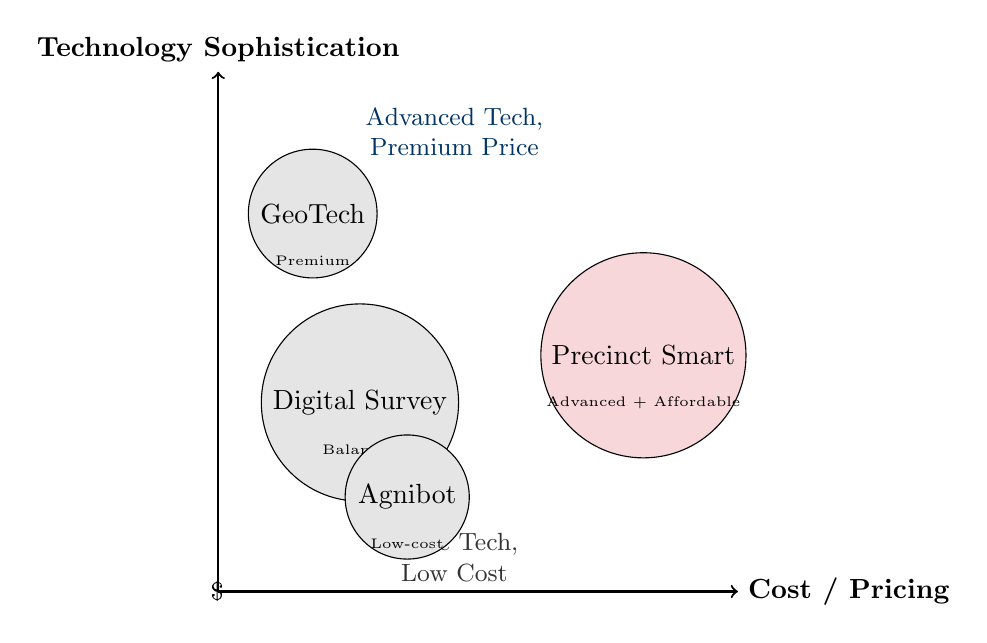
\begin{tikzpicture}[scale=1.2]
    % Axes
    \draw[thick, ->] (0,0) -- (5.5,0) node[right] {\textbf{Cost / Pricing}};
    \draw[thick, ->] (0,0) -- (0,5.5) node[above] {\textbf{Technology Sophistication}};

    % Quadrant labels
    \node at (2.5, 5) {\small \textcolor{PrimaryBlue}{Advanced Tech,}};
    \node at (2.5, 4.7) {\small \textcolor{PrimaryBlue}{Premium Price}};

    \node at (2.5, 0.5) {\small \textcolor{DarkGrey}{Basic Tech,}};
    \node at (2.5, 0.2) {\small \textcolor{DarkGrey}{Low Cost}};

    % Competitor positions
    \node[draw, circle, fill=AccentGreen!20] at (4.5, 2.5) {Precinct Smart};
    \node at (4.5, 2) {\tiny Advanced + Affordable};

    \node[draw, circle, fill=gray!20] at (1, 4) {GeoTech};
    \node at (1, 3.5) {\tiny Premium};

    \node[draw, circle, fill=gray!20] at (1.5, 2) {Digital Survey};
    \node at (1.5, 1.5) {\tiny Balanced};

    \node[draw, circle, fill=gray!20] at (2, 1) {Agnibot};
    \node at (2, 0.5) {\tiny Low-cost};

    % Center point
    \node at (0, 0) {\small \$};
\end{tikzpicture}

\vspace{1cm}

The position in the \textbf{upper-left quadrant} (advanced technology + affordable pricing) is defensible and attractive to all market segments.

\section{Go-to-Market Strategy}

\subsection{Phase 1: Government \& Infrastructure (Months 1-6)}

\textbf{Rationale:} Large budgets, long-term contracts, credibility builder

\begin{itemize}
    \item Target: Ministry of Land, LGED, Disaster Management Authority
    \item Strategy: Direct B2B sales with decision-makers
    \item Proof Points: Partner with university for feasibility pilot
    \item Expected Projects: 2-3 large government surveys
    \item Timeline to First Revenue: Month 4-6
\end{itemize}

\subsection{Phase 2: Real Estate \& Development (Months 6-12)}

\textbf{Rationale:} Recurring project demand, premium pricing capacity

\begin{itemize}
    \item Target: Major developers, construction companies
    \item Strategy: Showcase portfolio; offer pilot at reduced rates
    \item Proof Points: 3D visualization capabilities, accuracy credentials
    \item Expected Projects: 3-5 real estate projects
    \item Timeline to First Revenue: Month 7-9
\end{itemize}

\subsection{Phase 3: NGO \& Farmer Channel (Months 9-18)}

\textbf{Rationale:} Scale through existing NGO networks

\begin{itemize}
    \item Target: BRAC, ASA, Practical Action partnerships
    \item Strategy: Revenue-sharing model; farmer value demonstration
    \item Proof Points: Case studies showing yield improvement
    \item Expected Farmers Reached: 5K in Year 1, 50K by Year 3
    \item Timeline to First Contracts: Month 12-15
\end{itemize}

\section{Differentiation Strategy}

\subsection{Why Customers Will Choose Precinct Smart}

% Competitive Differentiation Matrix — TikZ grid
\begin{figure}[H]
    \centering
    \begin{tikzpicture}[x=1cm,y=0.85cm]
        % Header
        \fill[PrimaryBlue] (0,0) rectangle (13.5,0.85);
        \foreach \xpos/\lbl in {
            0.1/{Factor},
            2.8/{Competitors},
            6.3/{Precinct Smart},
            10.2/{Customer Benefit}}{
            \node[text=white,font=\bfseries\small,anchor=west] at (\xpos,0.425) {\lbl};
        }
        % Rows
        \foreach \row/\fac/\comp/\us/\ben in {
            1/{Technology}/{Photo + LiDAR}/{LiDAR + Photo + Data Science}/{Better accuracy + insights},
            2/{Pricing}/{Premium (10--15\% above)}/{Value-based}/{Better ROI},
            3/{Applications}/{Raw data only}/{Data + Apps + Consulting}/{Complete solution},
            4/{NGO Partnerships}/{None}/{Strategic focus}/{Farmer access},
            5/{Innovation}/{Stable, incremental}/{Rapid iteration}/{Future-proof},
            6/{Customer Service}/{Transactional}/{Partnership-oriented}/{Long-term relationship}
        }{
            \pgfmathsetmacro{\ybot}{-(\row-1)*0.85}
            \pgfmathsetmacro{\ytop}{\ybot+0.85}
            \ifodd\row
                \fill[LightGrey!60] (0,\ybot) rectangle (13.5,\ytop);
            \fi
            \draw[MidGrey!50] (0,\ybot) -- (13.5,\ybot);
            \node[anchor=west,font=\small\bfseries,text=PrimaryBlue] at (0.1,\ybot+0.425) {\fac};
            \node[anchor=west,font=\small,text=DarkGrey,text width=3.3cm] at (2.8,\ybot+0.425) {\comp};
            \node[anchor=west,font=\small\bfseries,text=AccentGreen,text width=3.7cm] at (6.3,\ybot+0.425) {\us};
            \node[anchor=west,font=\small,text=SecondaryBlue,text width=3.0cm] at (10.2,\ybot+0.425) {\ben};
        }
        \draw[PrimaryBlue,thick] (0,-5.1) rectangle (13.5,0.85);
        \foreach \xd in {2.75,6.25,10.15}{
            \draw[MidGrey!70] (\xd,-5.1) -- (\xd,0.85);
        }
    \end{tikzpicture}
    \caption{Competitive Differentiation Matrix}
    \label{tab:differentiation}
\end{figure}

\section{Competitive Response Strategies}

\subsection{If Competitors Lower Prices}

\textbf{Response:} Emphasize quality and long-term value
\begin{itemize}
    \item Highlight accuracy advantages (LiDAR precision)
    \item Showcase successful case studies
    \item Invest in brand and thought leadership
    \item Avoid price war; focus on value
\end{itemize}

\subsection{If Competitors Adopt LiDAR}

\textbf{Response:} Maintain technology lead through innovation
\begin{itemize}
    \item Integrate Data Science capabilities (they lack this)
    \item Expand custom application offerings
    \item Deepen NGO partnerships
    \item Invest in R\&D for next-gen capabilities
\end{itemize}

\subsection{If New Competitors Enter}

\textbf{Response:} Build switching costs
\begin{itemize}
    \item Lock in customers with custom applications
    \item Establish NGO partnerships (hard to replicate)
    \item Develop proprietary algorithms and datasets
    \item Invest in customer relationships and reputation
\end{itemize}

% ============================================================================
% END OF CHAPTER 5
% ============================================================================


% Chapter 6: Risks & Challenges
% ============================================================================
% CHAPTER 6: RISKS, CHALLENGES & MITIGATION
% ============================================================================

\chapter{Risks, Challenges \& Mitigation Strategies}

\section{Critical Business Risks}

\begin{table}[H]
    \centering
    \caption{Risk Assessment \& Mitigation Strategies}
    \label{tab:risk_assessment}
    \renewcommand{\arraystretch}{1.4}
    \begin{tabularx}{\textwidth}{>{\bfseries}p{3.2cm} | X | >{\bfseries\centering\arraybackslash}p{1.8cm} | X}
        \hline
        \theader{Risk} & \theader{Impact} & \theader{Probability} & \theader{Mitigation} \\
        \hline
        \textcolor{PrimaryBlue}{CAAB regulatory delays} & 3--6 month operational halt & \textcolor{AccentRed}{High} & Start licensing immediately; engage regulatory consultant \\
        \hline
        \textcolor{PrimaryBlue}{Monsoon weather impact} & 40\% of year non-flyable & \textcolor{AccentRed}{High} & Multi-region operations; seasonal project scheduling \\
        \hline
        \textcolor{PrimaryBlue}{Equipment malfunction} & Project delays, client loss & \textcolor{AccentOrange}{Medium} & Backup drone policy; dedicated maintenance fund \\
        \hline
        \textcolor{PrimaryBlue}{Market adoption slow} & Revenue below projections & \textcolor{AccentOrange}{Medium} & Focus on high-value government contracts first \\
        \hline
        \textcolor{PrimaryBlue}{Talent shortage} & Cannot scale operations & \textcolor{AccentOrange}{Medium} & Remote hiring; university partnerships; internal training \\
        \hline
        \textcolor{PrimaryBlue}{Competitive price war} & Margin compression & \textcolor{AccentRed}{High} & Differentiate on LiDAR technology + applications layer \\
        \hline
        \textcolor{PrimaryBlue}{Data security breach} & Loss of client trust & \textcolor{AccentGreen}{Low} & ISO 27001 compliance; end-to-end encrypted storage \\
        \hline
    \end{tabularx}
\end{table}

\section{Operational Challenges}

\subsection{Challenge 1: Weather \& Seasonality}

\textbf{Problem:} Bangladesh experiences 4-month monsoon (June-September) with heavy rains

\textbf{Impact:}
\begin{itemize}
    \item 40\% of year unsuitable for flying
    \item Projects must be scheduled in dry season (October-May)
    \item Delays in monsoon season projects
\end{itemize}

\textbf{Solutions:}
\begin{enumerate}
    \item Plan projects in dry season (6-month planning window)
    \item Build 3-4 month buffer into project timelines
    \item Geographic diversification (coastal areas less monsoon-affected)
    \item Develop covered/indoor mapping capabilities for special cases
    \item Offer year-round other services (consulting, data processing)
\end{enumerate}

\subsection{Challenge 2: Regulatory Compliance}

\textbf{Problem:} CAAB approval can take 2-3 months; no clear precedent for LiDAR operations

\textbf{Impact:}
\begin{itemize}
    \item Potential 3-month delay before first flight
    \item Uncertain approval timeline
    \item May require special permissions for certain operations
\end{itemize}

\textbf{Solutions:}
\begin{enumerate}
    \item Engage CAAB regulatory consultant immediately (Month 0)
    \item Apply for operations in phases/zones rather than national
    \item Build relationship with Survey of Bangladesh early
    \item Budget BDT 15 lakhs specifically for compliance
    \item Draft contingency applications to multiple agencies
    \item Plan for parallel development work during approval wait
\end{enumerate}

\subsection{Challenge 3: Skilled Workforce Shortage}

\textbf{Problem:} Bangladesh has limited GIS professionals and certified drone pilots

\textbf{Impact:}
\begin{itemize}
    \item Difficulty finding experienced GIS analysts
    \item Limited pool of certified drone pilots
    \item High salary competition
    \item Retention challenges
\end{itemize}

\textbf{Solutions:}
\begin{enumerate}
    \item Train pilots internally (50 flight hour requirement achievable in 2-3 months)
    \item Partner with universities (BUET, Jahangirnagar University) for recruitment and training
    \item Hire experienced remote contractors for specialized work
    \item Invest in 1-2 months intensive training for new team members
    \item Offer equity or profit-sharing to key staff
    \item Create clear career progression pathways
\end{enumerate}

\subsection{Challenge 4: High Equipment Costs}

\textbf{Problem:} BDT 100+ lakhs investment needed upfront; equipment costs are primary hurdle

\textbf{Impact:}
\begin{itemize}
    \item High capital requirement limits business scale
    \item Equipment becomes obsolete (every 3-4 years)
    \item Risk if equipment damaged or lost
\end{itemize}

\textbf{Solutions:}
\begin{enumerate}
    \item Consider equipment leasing initially instead of purchase
    \item Start with 1 drone + 1 LiDAR (BDT 40-50 lakhs)
    \item Scale up equipment after first 3-5 projects (ROI expected)
    \item Equipment insurance covers loss/damage
    \item Partner for equipment sharing with complementary vendors
    \item Apply for government procurement discounts/partnerships
\end{enumerate}

\subsection{Challenge 5: Market Education}

\textbf{Problem:} Most potential clients don't understand LiDAR value; may prefer photogrammetry

\textbf{Impact:}
\begin{itemize}
    \item Longer sales cycles (6-12 months)
    \item Higher customer acquisition costs
    \item Clients may default to cheaper alternatives
\end{itemize}

\textbf{Solutions:}
\begin{enumerate}
    \item Conduct free or discounted pilot surveys to demonstrate value
    \item Create compelling case studies from initial projects
    \item Partner with respected institutions (universities, major NGOs) for credibility
    \item Educate through government relationships and workshops
    \item Develop thought leadership content (blogs, whitepapers)
    \item Invest in marketing to build brand awareness
\end{enumerate}

\section{Financial Risk Management}

\subsection{Burn Rate Analysis}

\textbf{Monthly Operating Cost (Year 1):} BDT 2.3 lakhs

\textbf{Runway Analysis:}
\begin{itemize}
    \item Capital: BDT 100-125 lakhs
    \item Monthly burn: BDT 2.3 lakhs
    \item Runway: 43-54 months (good cushion)
    \item Break-even: Month 10 (provides safety margin)
\end{itemize}

\subsection{Cash Flow Management}

\textbf{Risk:} Large upfront equipment costs with delayed revenue

\textbf{Mitigation:}
\begin{enumerate}
    \item 50\% project deposit on initiation (covers equipment)
    \item 25\% progress payment on data delivery
    \item 25\% final payment on report (due within 15 days)
    \item Maintain 6-month operating expense buffer
    \item Don't overspend before break-even
    \item Seek advance payments for multi-project contracts
\end{enumerate}

\subsection{Revenue Risk}

\textbf{Scenario:} Actual revenue 50\% lower than projections (BDT 15L vs 30L in Year 1)

\textbf{Mitigation:}
\begin{enumerate}
    \item Reduce staffing to 8 (instead of 12)
    \item Operate from single hub (Dhaka only)
    \item Focus on high-margin consulting work
    \item Seek investor support or bank line of credit
    \item Adjust timeline expectations (break-even in Month 18-24)
    \item Maintain contingency budget for 6 additional months
\end{enumerate}

\section{Strategic Risks}

\subsection{Technology Obsolescence}

\textbf{Risk:} Rapid advancement in drone/sensor technology

\textbf{Mitigation:}
\begin{itemize}
    \item Allocate 5-10\% of revenue to R\&D
    \item Maintain partnerships with equipment vendors
    \item Train team on emerging technologies
    \item Build modular software architecture for easy updates
\end{itemize}

\subsection{Competition from Established Players}

\textbf{Risk:} GeoTech or other competitors adopt LiDAR + ML

\textbf{Mitigation:}
\begin{itemize}
    \item Build first-mover advantage through market share
    \item Develop proprietary algorithms and datasets
    \item Strengthen NGO and government partnerships
    \item Continuous innovation and feature development
    \item Brand building and thought leadership
\end{itemize}

\section{Mitigation Investment Summary}

% Risk Mitigation Budget — pgf-pie
\begin{figure}[H]
    \centering
    \begin{tikzpicture}
        \pie[
            radius=3.0,
            color={SecondaryBlue!80, AccentOrange!70, AccentGreen!65,
                   AccentRed!55, PrimaryBlue!60, MidGrey!80},
            text=legend,
            style={drop shadow},
            before number=\phantom{},
            after number=\%,
            sum=63
        ]{
            15/Regulatory consulting \& licensing (BDT 15L),
            10/Backup equipment fund (BDT 10L),
            5/Team training \& development (BDT 5L),
            8/Insurance -- liability \& equipment (BDT 8L),
            15/Working capital buffer -- 6 months (BDT 15L),
            10/Contingency reserve (BDT 10L)
        }
    \end{tikzpicture}
    \caption{Risk Mitigation Budget Allocation (Total: BDT 63 Lakhs)}
    \label{tab:risk_budget}
\end{figure}

% ============================================================================
% END OF CHAPTER 6
% ============================================================================


% Chapter 7: Regional Delivery Plan
% ============================================================================
% CHAPTER 7: REGIONAL SERVICE DELIVERY PLAN
% ============================================================================

\chapter{Regional Service Delivery Plan}

\section{Regional Strategy Overview}

The expansion plan is straightforward: start where the revenue is strongest, prove the model, then push outward. Dhaka comes first, Chittagong follows in Month 3, and Khulna and Sylhet open in Years 2 and 3 as revenue supports the investment.

\section{Region 1: Dhaka \& Central (Priority 1 - Year 1)}

\subsection{Geographic Coverage}

Dhaka and its satellite cities --- Narayanganj, Gazipur, Tangail --- form the country's primary economic engine, with the highest concentration of government agencies, real estate developers, and infrastructure projects.

\subsection{Market Characteristics}

\begin{itemize}
    \item \textbf{Key Clients:}
    \begin{itemize}
        \item Dhaka City Corporation
        \item Major real estate developers (BASHUNDHARA, Nasha, Concord)
        \item Government ministries (Land, Public Works, Disaster Management)
        \item International development organizations (ADB, World Bank projects)
    \end{itemize}

    \item \textbf{Service Demand:}
    \begin{itemize}
        \item Urban planning \& infrastructure mapping
        \item Real estate site selection
        \item Land survey \& documentation
        \item Building footprint extraction
        \item Infrastructure project design support
    \end{itemize}

    \item \textbf{Market Size:} BDT 40-50 lakhs annual opportunity
\end{itemize}

\subsection{Implementation Timeline}

\begin{itemize}
    \item \textbf{Month 1:} Office setup, team hiring, equipment procurement
    \item \textbf{Month 2:} Regulatory approvals, pilot projects
    \item \textbf{Month 3:} Government project targeting begins
    \item \textbf{Month 6:} Real estate client acquisition starts
    \item \textbf{Month 12:} Establish operational excellence, expand to Region 2
\end{itemize}

\subsection{Success Metrics}

\begin{itemize}
    \item 5-8 projects completed
    \item 2-3 case studies for portfolio
    \item 5-10 government/corporate client relationships
    \item BDT 40-50 lakhs revenue
\end{itemize}

\section{Region 2: Chittagong \& Southeast (Priority 2 - Year 1)}

\subsection{Geographic Coverage}

Chittagong and the southeastern belt --- Cox's Bazar, Rangamati, Bandarban --- is Bangladesh's second economic centre, with terrain that makes LiDAR considerably more valuable than photogrammetry alone.

\subsection{Market Characteristics}

\begin{itemize}
    \item \textbf{Key Clients:}
    \begin{itemize}
        \item Chittagong Port Authority
        \item Tourism development agencies
        \item Hill tract development corporations
        \item Coastal/beach conservation projects
        \item Disaster management for cyclone preparedness
    \end{itemize}

    \item \textbf{Service Demand:}
    \begin{itemize}
        \item Port infrastructure mapping
        \item Coastal zone management
        \item Tourism site planning
        \item Forest inventory (hill tracts)
        \item Landslide risk mapping
        \item Cyclone flood modeling
    \end{itemize}

    \item \textbf{Unique Capability:} Hilly terrain is where LiDAR earns its premium. Photogrammetry struggles with dense vegetation and complex elevation; LiDAR cuts through both.

    \item \textbf{Market Size:} BDT 20-25 lakhs annual opportunity
\end{itemize}

\subsection{Implementation Timeline}

\begin{itemize}
    \item \textbf{Month 3:} Regional hub opening in Chittagong
    \item \textbf{Month 4:} Port Authority project targeting
    \item \textbf{Month 6:} Hilltract survey pilot projects
    \item \textbf{Month 12:} Established regional presence
\end{itemize}

\subsection{Success Metrics}

\begin{itemize}
    \item 5-8 projects (mix of government and private)
    \item Specialized hill-terrain expertise demonstrated
    \item BDT 20-25 lakhs revenue
    \item Regional hub established with 3-4 staff
\end{itemize}

\section{Region 3: Khulna \& Southwest (Priority 3 - Year 2)}

\subsection{Geographic Coverage}

The southwest delta --- Khulna, Barisal, Satkhira, Jessore --- is agricultural heartland and home to the NGO networks that make the farmer application platform viable.

\subsection{Market Characteristics}

\begin{itemize}
    \item \textbf{Key Clients:}
    \begin{itemize}
        \item Agricultural cooperatives \& farming groups
        \item Shrimp farming operations
        \item Sundarbans management authority
        \item NGOs in development and conservation
        \item Environmental research institutions
    \end{itemize}

    \item \textbf{Service Demand:}
    \begin{itemize}
        \item Precision agriculture mapping
        \item Crop health monitoring (NDVI)
        \item Land use classification
        \item Water resource mapping
        \item Soil health assessment
        \item Mangrove/Sundarbans monitoring
    \end{itemize}

    \item \textbf{Unique Advantage:} BRAC, ASA, and Practical Action operate heavily here. Those existing networks become the distribution channel for the farmer apps.

    \item \textbf{Market Size:} BDT 30-35 lakhs annual opportunity
\end{itemize}

\subsection{Implementation Timeline}

\begin{itemize}
    \item \textbf{Month 6, Y2:} Regional hub opening in Khulna
    \item \textbf{Month 9, Y2:} NGO partnership pilots begin
    \item \textbf{Month 12, Y2:} First 5K farmers on Data Science platform
    \item \textbf{Month 18, Y2:} Expanded partnership with 2-3 NGOs
\end{itemize}

\subsection{Success Metrics}

\begin{itemize}
    \item 10-15 projects
    \item 5K+ farmers reached through NGO channels
    \item 2-3 NGO strategic partnerships
    \item BDT 30-35 lakhs revenue
    \item Regional hub with 3-4 staff
\end{itemize}

\section{Region 4: Sylhet \& Northeast (Priority 4 - Year 3)}

\subsection{Geographic Coverage}

Sylhet, Moulvibazar, Sunamganj --- tea country. The focus here is research partnerships, speciality crop monitoring, and biodiversity work.

\subsection{Market Characteristics}

\begin{itemize}
    \item \textbf{Key Clients:}
    \begin{itemize}
        \item Tea garden operators (80+ major estates)
        \item Forest research institutions
        \item Climate adaptation projects
        \item Agricultural universities
        \item Environmental research centers
    \end{itemize}

    \item \textbf{Service Demand:}
    \begin{itemize}
        \item Tea plantation health monitoring
        \item Forest inventory \& conservation
        \item Climate vulnerability mapping
        \item Agricultural research data
        \item Ecosystem monitoring
        \item Species mapping
    \end{itemize}

    \item \textbf{Unique Focus:} Research partnerships; specialized crops (tea); biodiversity

    \item \textbf{Market Size:} BDT 15-20 lakhs annual opportunity
\end{itemize}

\subsection{Implementation Timeline}

\begin{itemize}
    \item \textbf{Month 6, Y3:} Regional hub opening (partnered model)
    \item \textbf{Month 9, Y3:} Tea estate survey projects
    \item \textbf{Month 12, Y3:} Research partnerships established
\end{itemize}

\subsection{Success Metrics}

\begin{itemize}
    \item 5-8 projects
    \item Tea plantation monitoring platform established
    \item 2-3 research partnerships
    \item BDT 15-20 lakhs revenue
    \item Regional presence with 2-3 staff
\end{itemize}

\section{Regional Hub Expansion Timeline}

\begin{table}[h!]
    \centering
    \caption{Regional Hub Development Schedule}
    \label{tab:hub_expansion}
    \begin{tabularx}{\textwidth}{l | X | X | X | X}
        \hline
        \theader{Region} & \theader{Launch} & \theader{Staff} & \theader{Investment} & \theader{Revenue Target} \\
        \hline
        Dhaka (HQ) & M1, Y1 & 8-10 & 50L & 40-50L \\
        \hline
        Chittagong & M3, Y1 & 3-4 & 15L & 20-25L \\
        \hline
        Khulna & M6, Y2 & 3-4 & 15L & 30-35L \\
        \hline
        Sylhet & M6, Y3 & 2-3 & 10L & 15-20L \\
        \hline
        \textbf{TOTAL} & & \textbf{16-21} & \textbf{90L} & \textbf{105-130L} \\
        \hline
    \end{tabularx}
\end{table}

\section{Inter-Regional Synergies}

\subsection{Knowledge Sharing}

\begin{itemize}
    \item Consistent operating procedures across all four hubs mean a project team from Dhaka can plug into a Chittagong job without a learning curve
    \item Learnings from each project type flow back to all hubs through monthly team reviews
    \item All heavy data processing runs through Dhaka, keeping infrastructure costs consolidated
\end{itemize}

\subsection{Equipment Sharing}

\begin{itemize}
    \item Drone units travel --- a busy period in Dhaka doesn't leave Chittagong grounded
    \item Processing workloads are balanced across hubs based on capacity
    \item Backup equipment is shared across the network for redundancy
\end{itemize}

\subsection{Project Allocation}

\begin{itemize}
    \item Large national projects coordinated across hubs
    \item Regional specialists support neighboring regions
    \item Emergency response (cyclones, disasters) coordinated nationally
\end{itemize}

% ============================================================================
% END OF CHAPTER 7
% ============================================================================


% Chapter 8: ML & Farmer Apps
% ============================================================================
% CHAPTER 8: Data Science & FARMER-LEVEL APPLICATION ROADMAP
% ============================================================================

\chapter{ML \& Farmer-Level Application Roadmap}

\section{Parallel Development Strategy (Year 1-2)}

Most GIS companies in Bangladesh stop at handing over a dataset. Precinct Smart is building the full pipeline: from drone flights and LiDAR point clouds, through machine learning models, to farmer-facing applications delivered through NGO distribution networks. The survey business and the platform develop simultaneously --- Year 1 is not a waiting period for the apps.

\textbf{Objective:} Build a LiDAR + photogrammetry + data science platform that turns field observations into actionable farmer-level insights, distributed at scale through NGO partnerships.

\section{Core Data Science Applications}

\subsection{APP 1: Crop Health Monitor}

\subsubsection{Technology Stack}

\begin{itemize}
    \item \textbf{Input Data:} NDVI (Normalized Difference Vegetation Index) from drone RGB imagery
    \item \textbf{ML Model:} Convolutional Neural Networks (CNN) for pattern recognition
    \item \textbf{Prediction:} Disease/pest outbreak prediction using historical data
    \item \textbf{Platform:} WhatsApp/SMS alerts + mobile app (low-bandwidth)
\end{itemize}

\subsubsection{Features}

\begin{enumerate}
    \item \textbf{Real-time Crop Health Index (0-100 scale)}
        \begin{itemize}
            \item Green = Healthy
            \item Yellow = Caution
            \item Red = Problem (pest/disease/water stress)
        \end{itemize}

    \item \textbf{Disease/Pest Outbreak Prediction}
        \begin{itemize}
            \item Data Science model trained on 5+ years historical data
            \item Predicts outbreak 7-14 days in advance
            \item Accuracy target: 75-80\%
        \end{itemize}

    \item \textbf{Optimal Harvest Timing Recommendation}
        \begin{itemize}
            \item Predict best harvest date within 3-day window
            \item Maximize yield and quality
        \end{itemize}

    \item \textbf{Water Stress Detection}
        \begin{itemize}
            \item Identify fields needing irrigation
            \item Optimize water use (critical in Bangladesh with water stress)
        \end{itemize}
\end{enumerate}

\subsubsection{Farmer Interface}

\begin{itemize}
    \item \textbf{Primary:} WhatsApp alerts (simple, no app download needed)
    \item \textbf{Secondary:} SMS for low-bandwidth areas
    \item \textbf{Advanced:} Mobile app for farmers with smartphones
    \item \textbf{NGO Portal:} Aggregated data for program managers
\end{itemize}

\subsubsection{Commercial Model}

\textbf{Pricing:} BDT 500-1,000 per farmer per season

\textbf{Example Revenue:}
\begin{itemize}
    \item 100 farmers × BDT 750/season = BDT 75,000/season
    \item 2 seasons/year = BDT 150,000/year
    \item Scale to 5,000 farmers = BDT 7.5M/year by Year 3
\end{itemize}

\textbf{Development Timeline:} Month 6-12 (Year 1)

\textbf{MVP Features:} Health monitoring + disease alert (Months 6-9)

\textbf{Full Feature Release:} Add harvest timing + water stress (Months 10-12)

\subsection{APP 2: Yield Predictor}

\subsubsection{Technology}

\begin{itemize}
    \item \textbf{ML Model:} Random Forest or XGBoost (tabular data)
    \item \textbf{Input Variables:} Soil type, elevation (from LiDAR), weather, crop variety, farmer practices
    \item \textbf{Integration:} Weather API (IMD, NASA POWER), soil database, yield history
    \item \textbf{Accuracy Target:} 85-90\%
\end{itemize}

\subsubsection{Features}

\begin{enumerate}
    \item \textbf{Pre-season Yield Estimation}
        \begin{itemize}
            \item Predict yield (tons/hectare) before planting
            \item Help farmers make variety selection
            \item Inform input purchasing decisions
        \end{itemize}

    \item \textbf{Weather Impact Forecasting}
        \begin{itemize}
            \item Model impact of forecasted weather on yield
            \item Alert farmers to weather risks
            \item Recommend adaptation strategies
        \end{itemize}

    \item \textbf{Optimal Input Recommendation}
        \begin{itemize}
            \item Fertilizer requirements (N:P:K)
            \item Water requirement (irrigation schedule)
            \item Seed variety recommendations
            \item Planting date optimization
        \end{itemize}

    \item \textbf{Market Price Prediction}
        \begin{itemize}
            \item Predict crop prices at harvest time
            \item Help farmers decide storage vs. immediate sale
            \item Inform crop selection decisions
        \end{itemize}
\end{enumerate}

\subsubsection{Commercial Model}

\textbf{Revenue Model:} Subscription through NGO partnerships

\textbf{Pricing:} BDT 2,000-5,000 per farmer per season

\textbf{Scale Opportunity:}
\begin{itemize}
    \item 5,000 farmers × BDT 3,000 = BDT 15M/year by Year 3
\end{itemize}

\textbf{Development Timeline:} Month 12-18 (Year 2)

\subsection{APP 3: Land Planning Assistant}

\subsubsection{Technology}

\begin{itemize}
    \item \textbf{Data Sources:} LiDAR elevation, soil classification, water availability
    \item \textbf{ML Model:} Decision tree for crop suitability classification
    \item \textbf{Analysis:} Erosion risk, flood susceptibility, drought vulnerability
\end{itemize}

\subsubsection{Features}

\begin{enumerate}
    \item \textbf{Best Crops for Your Land}
        \begin{itemize}
            \item Data Science model recommends suitable crops based on:
            \begin{itemize}
                \item Soil type and pH
                \item Elevation and slope
                \item Water availability
                \item Climate zone
            \end{itemize}
        \end{itemize}

    \item \textbf{Slope-based Erosion Risk Mapping}
        \begin{itemize}
            \item LiDAR elevation used to calculate slopes
            \item Identify erosion-prone areas
            \item Recommend soil conservation measures
        \end{itemize}

    \item \textbf{Irrigation Planning}
        \begin{itemize}
            \item Calculate water requirement per crop
            \item Identify surface water availability
            \item Estimate groundwater feasibility
            \item Optimize water infrastructure investment
        \end{itemize}

    \item \textbf{Land Rotation Recommendations}
        \begin{itemize}
            \item Suggest crop rotation schedule
            \item Maintain soil fertility
            \item Reduce pest/disease pressure
        \end{itemize}
\end{enumerate}

\subsubsection{Farmer Interface}

\begin{itemize}
    \item \textbf{Web Portal:} Detailed analysis and maps
    \item \textbf{Printed Field Maps:} 1:2000 scale maps with recommendations
    \item \textbf{NGO Consultation:} Field agent visits with recommendations
\end{itemize}

\subsubsection{Commercial Model}

\textbf{Revenue Model:} One-time consulting fee per farm

\textbf{Pricing:} BDT 10,000-15,000 per farm (covers 2-5 hectares)

\textbf{Scale Opportunity:}
\begin{itemize}
    \item 2,000 farms × BDT 12,500 = BDT 2.5M/year by Year 3
\end{itemize}

\textbf{Development Timeline:} Month 9-15 (Year 2)

\section{NGO Partnership Model}

\subsection{How It Works}

The model works as a chain:

\begin{enumerate}
    \item \textbf{Precinct Smart} collects LiDAR + RGB imagery
    \item \textbf{Data Processing} with Data Science algorithms
    \item \textbf{Actionable Insights} generated (crop health, yield predictions, planning)
    \item \textbf{NGO Distribution} reaches farmers via existing channels
    \item \textbf{Farmer Decision-Making} improves (better productivity)
    \item \textbf{Revenue Sharing:} 60\% to NGO, 40\% to Precinct Smart
\end{enumerate}

\subsection{Target NGO Partners}

\begin{table}[h!]
    \centering
    \caption{Potential NGO Partners \& Reach}
    \label{tab:ngo_partners}
    \begin{tabularx}{\textwidth}{l | X | X}
        \hline
        \theader{NGO} & \theader{Members/Farmers} & \theader{Relevant Programs} \\
        \hline
        BRAC & 10M+ & Agriculture, climate adaptation, youth \\
        \hline
        ASA & 2M+ & Microfinance, agricultural loans \\
        \hline
        Practical Action & 500K+ & Climate adaptation, agriculture \\
        \hline
        RDRS Bangladesh & 200K+ & Agricultural development \\
        \hline
        GK Trust & 300K+ & Development services \\
        \hline
    \end{tabularx}
\end{table}

\subsection{Partnership Approach}

\textbf{Phase 1 (Year 1):} One NGO, one region, 500--1,000 farmers. The product is limited to crop health monitoring. The goal is to prove that farmers will pay and that the NGO channel actually works --- before scaling either.

\textbf{Phase 2 (Year 2):} Three to four NGOs, full product suite, 5,000--10,000 farmers across multiple regions. Real impact metrics start to accumulate, and the subscription revenue line becomes meaningful.

\textbf{Phase 3 (Year 3):} National scale --- 50,000+ farmers, integration with government agricultural programs, and subscription revenue that no longer requires proportional cost growth to maintain.

\subsection{Impact Metrics}

The platform targets a 15\% average yield improvement by Year 2, rising to 20--25\% income improvement by Year 3 as price optimization tools layer on top. Impact is measured concretely: baseline surveys before program entry, annual household income assessments, crop productivity data from drone surveys, and farmer satisfaction tracking. This is not speculative --- 127,500 farmers are already adopting drone technology and reporting yield improvements of 15--60\%.

\section{ML Platform Revenue Potential}

\begin{table}[h!]
    \centering
    \caption{ML App Revenue Projections (Year 2-3)}
    \label{tab:ml_revenue}
    \begin{tabularx}{\textwidth}{l | X | X}
        \hline
        \theader{App} & \theader{Year 2 Revenue} & \theader{Year 3 Revenue} \\
        \hline
        Crop Health Monitor & BDT 5L & BDT 15L \\
        \hline
        Yield Predictor & BDT 2L & BDT 10L \\
        \hline
        Land Planning Assistant & BDT 1L & BDT 5L \\
        \hline
        \textbf{TOTAL Data Science REVENUE} & \textbf{BDT 8L} & \textbf{BDT 30L} \\
        \hline
        As \% of Total Revenue & 8\% & 15\% \\
        \hline
    \end{tabularx}
\end{table}

\section{Technical Development Approach}

\subsection{ML Development Stack}

\begin{itemize}
    \item \textbf{Languages:} Python (scikit-learn, TensorFlow)
    \item \textbf{Data Processing:} Pandas, NumPy, GDAL
    \item \textbf{APIs:} Flask/FastAPI for backend services
    \item \textbf{Frontend:} React/Vue for web portal
    \item \textbf{Database:} PostgreSQL + PostGIS for spatial data
    \item \textbf{Cloud:} AWS SageMaker or Google Vertex AI for Data Science training
\end{itemize}

\subsection{Data Pipeline Architecture}

\begin{enumerate}
    \item \textbf{Data Collection:} Drone flights + satellite data
    \item \textbf{Data Processing:} Point cloud processing + image analysis
    \item \textbf{Feature Engineering:} Extract NDVI, elevation, slope, soil indicators
    \item \textbf{ML Model Training:} Retrain models quarterly with new data
    \item \textbf{Inference Pipeline:} Real-time predictions for farmers
    \item \textbf{Visualization:} Maps and charts in web/mobile interfaces
\end{enumerate}

% ============================================================================
% END OF CHAPTER 8
% ============================================================================


% Chapter 9: Implementation Timeline
% ============================================================================
% CHAPTER 9: IMPLEMENTATION TIMELINE
% ============================================================================

\chapter{36-Month Implementation Timeline}

\section{PHASE 1: Foundation (Months 1-3)}

\begin{table}[H]
    \centering
    \caption{Phase 1 Milestones \& Deliverables}
    \label{tab:phase1}
    \renewcommand{\arraystretch}{1.3}
    \begin{tabularx}{\textwidth}{l | X | X}
        \hline
        \theader{Month} & \theader{Milestone} & \theader{Deliverable} \\
        \hline
        \textbf{\textcolor{SecondaryBlue}{1}} & \textbf{\textcolor{PrimaryBlue}{Regulatory setup}} & CAAB application, business registration \\
        \hline
        \textbf{\textcolor{SecondaryBlue}{1--2}} & \textbf{\textcolor{PrimaryBlue}{Equipment procurement}} & 2 drones, 2 LiDAR sensors, servers \\
        \hline
        \textbf{\textcolor{SecondaryBlue}{2}} & \textbf{\textcolor{PrimaryBlue}{Team hiring}} & Ops manager, pilot, GIS analysts \\
        \hline
        \textbf{\textcolor{SecondaryBlue}{2--3}} & \textbf{\textcolor{PrimaryBlue}{Office setup}} & Dhaka headquarters operational \\
        \hline
        \textbf{\textcolor{SecondaryBlue}{3}} & \textbf{\textcolor{PrimaryBlue}{Pilot projects}} & 2--3 test surveys for portfolio \\
        \hline
    \end{tabularx}
\end{table}

\textbf{Expected Outcome:} By end of Month 3, the business is fully equipped, staffed, and cleared for operations --- ready for market launch.

\section{PHASE 2: Launch \& Market Entry (Months 4-12)}

\begin{table}[H]
    \centering
    \caption{Phase 2 Quarterly Milestones}
    \label{tab:phase2}
    \renewcommand{\arraystretch}{1.3}
    \begin{tabularx}{\textwidth}{l | X | X}
        \hline
        \theader{Period} & \theader{Focus} & \theader{Target} \\
        \hline
        \textbf{\textcolor{SecondaryBlue}{Q2 (M4--6)}} & \textbf{\textcolor{PrimaryBlue}{Dhaka launch}} & 5--8 projects, 2 case studies \\
        \hline
        \textbf{\textcolor{SecondaryBlue}{Q3 (M7--9)}} & \textbf{\textcolor{PrimaryBlue}{Chittagong hub}} & 5+ projects, hub operational \\
        \hline
        \textbf{\textcolor{SecondaryBlue}{Q4 (M10--12)}} & \textbf{\textcolor{PrimaryBlue}{Data Science app development}} & Crop Health Monitor MVP \\
        \hline
    \end{tabularx}
\end{table}

\noindent
\begin{minipage}[t]{0.48\textwidth}
    \begin{tcolorbox}[colback=BoxBlue,colframe=SecondaryBlue,arc=4pt,boxrule=1pt,
        halign=center,top=6pt,bottom=6pt]
        {\large\bfseries\color{PrimaryBlue}BDT 30L}\\[2pt]
        {\small\color{DarkGrey}Revenue Target}
    \end{tcolorbox}
\end{minipage}\hfill
\begin{minipage}[t]{0.48\textwidth}
    \begin{tcolorbox}[colback=BoxGreen,colframe=AccentGreen,arc=4pt,boxrule=1pt,
        halign=center,top=6pt,bottom=6pt]
        {\large\bfseries\color{AccentGreen}+BDT 2L}\\[2pt]
        {\small\color{DarkGrey}Expected Profit (Break-even)}
    \end{tcolorbox}
\end{minipage}

\section{PHASE 3: Growth \& Diversification (Months 13-24)}

\begin{table}[H]
    \centering
    \caption{Phase 3 Quarterly Milestones}
    \label{tab:phase3}
    \renewcommand{\arraystretch}{1.3}
    \begin{tabularx}{\textwidth}{l | X | X}
        \hline
        \theader{Period} & \theader{Focus} & \theader{Target} \\
        \hline
        \textbf{\textcolor{AccentGreen}{Q1--2 (M13--18)}} & \textbf{\textcolor{PrimaryBlue}{Scale services}} & 20 projects, 2--3 apps in beta \\
        \hline
        \textbf{\textcolor{AccentGreen}{Q2--3 (M16--21)}} & \textbf{\textcolor{PrimaryBlue}{Khulna hub launch}} & Start NGO pilots, 30+ projects \\
        \hline
        \textbf{\textcolor{AccentGreen}{Q4 (M22--24)}} & \textbf{\textcolor{PrimaryBlue}{Data Science expansion}} & Yield Predictor + Land Planner ready \\
        \hline
    \end{tabularx}
\end{table}

\noindent
\begin{minipage}[t]{0.32\textwidth}
    \begin{tcolorbox}[colback=BoxBlue,colframe=SecondaryBlue,arc=4pt,boxrule=1pt,
        halign=center,top=6pt,bottom=6pt]
        {\large\bfseries\color{PrimaryBlue}BDT 96.5L}\\[2pt]
        {\small\color{DarkGrey}Revenue Target}
    \end{tcolorbox}
\end{minipage}\hfill
\begin{minipage}[t]{0.32\textwidth}
    \begin{tcolorbox}[colback=BoxGreen,colframe=AccentGreen,arc=4pt,boxrule=1pt,
        halign=center,top=6pt,bottom=6pt]
        {\large\bfseries\color{AccentGreen}BDT 49.5L}\\[2pt]
        {\small\color{DarkGrey}Expected Profit}
    \end{tcolorbox}
\end{minipage}\hfill
\begin{minipage}[t]{0.32\textwidth}
    \begin{tcolorbox}[colback=BoxGreen,colframe=AccentGreen,arc=4pt,boxrule=1pt,
        halign=center,top=6pt,bottom=6pt]
        {\large\bfseries\color{AccentGreen}BDT 51.5L}\\[2pt]
        {\small\color{DarkGrey}Cumulative Profit}
    \end{tcolorbox}
\end{minipage}

\section{PHASE 4: Scaling \& Innovation (Months 25-36)}

\begin{table}[H]
    \centering
    \caption{Phase 4 Quarterly Milestones}
    \label{tab:phase4}
    \renewcommand{\arraystretch}{1.3}
    \begin{tabularx}{\textwidth}{l | X | X}
        \hline
        \theader{Period} & \theader{Focus} & \theader{Target} \\
        \hline
        \textbf{\textcolor{AccentOrange}{Q1--2 (M25--30)}} & \textbf{\textcolor{PrimaryBlue}{Sylhet hub launch}} & 50K farmers on platform \\
        \hline
        \textbf{\textcolor{AccentOrange}{Q3--4 (M31--36)}} & \textbf{\textcolor{PrimaryBlue}{Platform optimisation}} & 60+ projects/year, multi-NGO \\
        \hline
    \end{tabularx}
\end{table}

\noindent
\begin{minipage}[t]{0.32\textwidth}
    \begin{tcolorbox}[colback=BoxBlue,colframe=SecondaryBlue,arc=4pt,boxrule=1pt,
        halign=center,top=6pt,bottom=6pt]
        {\large\bfseries\color{PrimaryBlue}BDT 204L}\\[2pt]
        {\small\color{DarkGrey}Revenue Target}
    \end{tcolorbox}
\end{minipage}\hfill
\begin{minipage}[t]{0.32\textwidth}
    \begin{tcolorbox}[colback=BoxGreen,colframe=AccentGreen,arc=4pt,boxrule=1pt,
        halign=center,top=6pt,bottom=6pt]
        {\large\bfseries\color{AccentGreen}BDT 136L}\\[2pt]
        {\small\color{DarkGrey}Expected Profit}
    \end{tcolorbox}
\end{minipage}\hfill
\begin{minipage}[t]{0.32\textwidth}
    \begin{tcolorbox}[colback=BoxGreen,colframe=AccentGreen,arc=4pt,boxrule=1pt,
        halign=center,top=6pt,bottom=6pt]
        {\large\bfseries\color{AccentGreen}BDT 187.5L}\\[2pt]
        {\small\color{DarkGrey}Cumulative 3-Year Profit}
    \end{tcolorbox}
\end{minipage}

\section{Critical Path Items}

\begin{importantbox}
    These items sit on the critical path. A delay in any one of them cascades through everything else:
    \begin{enumerate}
        \item CAAB drone licensing (Months 1--2) --- \textbf{CRITICAL}: no flight without it
        \item Pilot certification (Months 1--2) --- \textbf{CRITICAL}: can run in parallel with licensing
        \item First client acquisition (Months 4--5) --- \textbf{CRITICAL}: break-even depends on it
        \item Government project approval (Months 4--6) --- \textbf{IMPORTANT}: establishes credibility early
        \item ML model training data collection (Months 6--9) --- \textbf{IMPORTANT}: feeds Year 2 app launch
    \end{enumerate}
\end{importantbox}

% ============================================================================
% END OF CHAPTER 9
% ============================================================================


% Chapter 10: KPIs
% ============================================================================
% CHAPTER 10: KEY PERFORMANCE INDICATORS
% ============================================================================

\chapter{Key Performance Indicators (KPIs)}

\section{Business KPIs}

\begin{table}[h!]
    \centering
    \caption{Business KPI Targets (Year 1-3)}
    \label{tab:business_kpis}
    \begin{tabularx}{\textwidth}{l | X | X | X}
        \hline
        \theader{KPI} & \theader{Year 1} & \theader{Year 2} & \theader{Year 3} \\
        \hline
        Projects Completed & 5-8 & 15-20 & 40-50 \\
        \hline
        Area Covered (sq. km) & 12-15 & 35-40 & 70-80 \\
        \hline
        Total Revenue (BDT L) & 30 & 96.5 & 204 \\
        \hline
        Gross Margin & 35\% & 55\% & 70\% \\
        \hline
        Net Profit (BDT L) & 2 & 49.5 & 136 \\
        \hline
        Customer Acquisition Cost & 5,000 & 4,000 & 3,000 \\
        \hline
        Customer Lifetime Value & 25,000 & 50,000 & 100,000 \\
        \hline
        Repeat Customer Rate & 40\% & 60\% & 75\% \\
        \hline
    \end{tabularx}
\end{table}

\section{Operational KPIs}

\begin{table}[h!]
    \centering
    \caption{Operational KPI Targets}
    \label{tab:operational_kpis}
    \begin{tabularx}{\textwidth}{l | X}
        \hline
        \theader{KPI} & \theader{Target} \\
        \hline
        Project On-time Delivery & >95\% \\
        \hline
        Data Accuracy (RMSE) & <10 cm (LiDAR), <5 cm (GPS) \\
        \hline
        Customer Satisfaction Score & >4.5/5.0 \\
        \hline
        Team Retention Rate & >90\% \\
        \hline
        Equipment Uptime & >90\% \\
        \hline
        Data Processing Time & <2 weeks \\
        \hline
        Safety Incidents & Zero \\
        \hline
    \end{tabularx}
\end{table}

\section{ML \& Farmer Impact KPIs}

\begin{table}[h!]
    \centering
    \caption{ML Platform \& Farmer Impact KPIs}
    \label{tab:farmer_impact_kpis}
    \begin{tabularx}{\textwidth}{l | X | X}
        \hline
        \theader{KPI} & \theader{Year 2} & \theader{Year 3} \\
        \hline
        Farmers on Platform & 5,000 & 50,000 \\
        \hline
        Crop Health Prediction Accuracy & 75\% & 85\% \\
        \hline
        Farmer Income Improvement & 15\% avg & 25\% avg \\
        \hline
        NGO Strategic Partners & 1 & 3-4 \\
        \hline
        Monthly Active Users & 2,000 & 15,000 \\
        \hline
        App Adoption Rate & 50\% & 75\% \\
        \hline
    \end{tabularx}
\end{table}

\section{Financial KPIs}

\begin{itemize}
    \item \textbf{Gross Margin:} 35\% → 70\% (improving efficiency)
    \item \textbf{Operating Expense Ratio:} 93\% → 33\% (operational leverage)
    \item \textbf{Return on Assets:} Year 1: 1.5\%, Year 3: 104\%
    \item \textbf{Break-even:} Month 10, Year 1
    \item \textbf{Payback Period:} 24 months (cumulative)
\end{itemize}

% ============================================================================
% END OF CHAPTER 10
% ============================================================================


% Chapter 11: Market Outlook
% ============================================================================
% CHAPTER 11: MARKET OUTLOOK & EXPANSION OPPORTUNITIES
% ============================================================================

\chapter{Market Outlook \& Expansion Opportunities (Year 3+)}

\section{Geographic Expansion Opportunities}

\subsection{Myanmar Market}

\textbf{Opportunity:} Similar agricultural and environmental context, less competition

\begin{itemize}
    \item Agricultural sector with 10M+ farmers
    \item Growing infrastructure investment
    \item Limited GIS service providers
    \item Estimated market size: USD 5-10M
\end{itemize}

\textbf{Timeline:} Year 4-5

\subsection{India (Northeast States)}

\textbf{Opportunity:} Similar climate and crops to Bangladesh northeast

\begin{itemize}
    \item Assam, Meghalaya, Manipur regions
    \item Tea and agriculture-focused
    \item Growing development initiatives
    \item Estimated market size: USD 10-20M
\end{itemize}

\textbf{Timeline:} Year 5+

\subsection{Southeast Asia Expansion}

\textbf{Opportunity:} Vietnam, Cambodia, Laos with similar agriculture and development needs

\textbf{Timeline:} Year 5-7

\section{Service Expansion Opportunities}

\subsection{Thermal Imaging Services}

Temperature-based crop and infrastructure monitoring

\textbf{Applications:}
\begin{itemize}
    \item Detect crop water stress via leaf temperature
    \item Infrastructure defect detection (bridges, dams)
    \item Disease spreading patterns
\end{itemize}

\textbf{Revenue Opportunity:} BDT 5-10 lakhs/year (Year 3+)

\subsection{Bathymetric Surveys}

Water depth mapping for fisheries and water management

\textbf{Applications:}
\begin{itemize}
    \item Fish farming pond mapping
    \item River navigation improvement
    \item Water resource assessment
    \item Coastal bathymetry
\end{itemize}

\textbf{Revenue Opportunity:} BDT 10-15 lakhs/year (Year 4+)

\subsection{Multispectral Analysis}

Beyond RGB and thermal - multiple wavelength bands

\textbf{Applications:}
\begin{itemize}
    \item Soil nutrient status detection
    \item Disease identification in early stages
    \item Water quality assessment
    \item Biomass estimation
\end{itemize}

\textbf{Revenue Opportunity:} BDT 15-20 lakhs/year (Year 3+)

\subsection{AI-Powered Feature Extraction}

Automated detection and classification of features

\textbf{Applications:}
\begin{itemize}
    \item Automatic building footprint extraction
    \item Road network detection
    \item Forest/tree counting and species classification
    \item Infrastructure network mapping
\end{itemize}

\textbf{Revenue Opportunity:} BDT 20-30 lakhs/year (Year 3+)

\section{Market Size Potential (Year 5+)}

\textbf{Conservative Scenario:}
\begin{itemize}
    \item Bangladesh only
    \item BDT 500 lakhs revenue
    \item BDT 300 lakhs profit
\end{itemize}

\textbf{Optimistic Scenario:}
\begin{itemize}
    \item Bangladesh + Myanmar + India Northeast
    \item BDT 1,000 lakhs revenue
    \item BDT 600 lakhs profit
\end{itemize}

\textbf{With NGO Scaling:}
\begin{itemize}
    \item 500K farmers on platform
    \item BDT 1,500+ lakhs revenue
    \item Significant social impact (500K farmers with 25\% income improvement)
\end{itemize}

% ============================================================================
% END OF CHAPTER 11
% ============================================================================


% Chapter 12: Investment Summary
% ============================================================================
% CHAPTER 12: INVESTMENT SUMMARY & FUNDING REQUIREMENTS
% ============================================================================

\chapter{Investment Summary \& Funding Requirements}

\section{Total Investment Needed}

\textcolor{AccentGreen}{\textbf{Total Startup Capital: BDT 100-125 lakhs (USD 120,000-150,000)}}

\subsection{Capital Allocation}

% Investment Capital Breakdown — pgf-pie
\begin{figure}[H]
    \centering
    \begin{tikzpicture}
        \pie[
            radius=3.2,
            color={SecondaryBlue!80, AccentGreen!70, AccentOrange!80, MidGrey!90},
            text=legend,
            style={drop shadow},
            before number=\phantom{},
            after number=\%,
            sum=100
        ]{
            75/Equipment \& Technology (75\%),
            7/Office \& Infrastructure (7\%),
            11/Regulatory \& Compliance (11\%),
            11/Working Capital (11\%)
        }
    \end{tikzpicture}
    \caption{Investment Capital Breakdown (BDT 120--140 Lakhs)}
    \label{tab:investment_breakdown}
\end{figure}

\noindent
\begin{minipage}[t]{0.48\textwidth}
    \begin{tcolorbox}[colback=BoxBlue,colframe=SecondaryBlue,arc=4pt,boxrule=1pt,
        top=6pt,bottom=6pt,left=8pt,right=8pt]
        \small
        \textbf{\textcolor{PrimaryBlue}{Capital Breakdown:}}\\[4pt]
        \textbf{Equipment \& Technology:} BDT 90--100L (73--80\%)\\
        \textbf{Office \& Infrastructure:} BDT 8--10L (6--8\%)\\
        \textbf{Regulatory \& Compliance:} BDT 12--15L (10--12\%)\\
        \textbf{Working Capital Buffer:} BDT 10--15L (8--12\%)
    \end{tcolorbox}
\end{minipage}\hfill
\begin{minipage}[t]{0.48\textwidth}
    \begin{tcolorbox}[colback=BoxGreen,colframe=AccentGreen,arc=4pt,boxrule=1pt,
        top=6pt,bottom=6pt,left=8pt,right=8pt,halign=center]
        {\large\bfseries\color{AccentGreen}BDT 120--140 Lakhs}\\[4pt]
        {\small\color{DarkGrey}Total Capital Required}\\[2pt]
        {\small\color{DarkGrey}Minimum recommended: BDT 100--125L}
    \end{tcolorbox}
\end{minipage}

\subsection{Capital Allocation Chart}

\begin{figure}[H]
    \centering
    \begin{tikzpicture}
        \pie[
            radius=3.2,
            color={SecondaryBlue!80, AccentGreen!70, AccentOrange!80, MidGrey!90},
            text=legend,
            style={drop shadow},
            before number=\phantom{},
            after number=\%,
            sum=100
        ]{
            75/Equipment \& Technology (75\%),
            7/Office \& Infrastructure (7\%),
            11/Regulatory \& Compliance (11\%),
            11/Working Capital (11\%)
        }
    \end{tikzpicture}
    \caption{Startup Capital Allocation (BDT 120--140 Lakhs)}
    \label{fig:capital_allocation}
\end{figure}

\section{Expected Returns (3-Year Horizon)}

% 3-Year Financial Returns — pgfplots grouped bar chart
\begin{figure}[H]
    \centering
    \begin{tikzpicture}
        \begin{axis}[
            ybar,
            bar width=20pt,
            width=0.85\textwidth,
            height=7cm,
            enlarge x limits=0.3,
            symbolic x coords={Year 1, Year 2, Year 3},
            xtick=data,
            xlabel={\textbf{Year}},
            ylabel={\textbf{BDT (Lakhs)}},
            ymin=0, ymax=230,
            ytick={0,50,100,150,200},
            grid=major,
            grid style={dotted,gray!40},
            legend style={at={(0.97,0.97)},anchor=north east,font=\small,
                          draw=MidGrey,fill=LightGrey},
            tick label style={font=\small},
            label style={font=\small\bfseries},
            title={\textbf{3-Year Financial Returns (BDT Lakhs)}},
            title style={font=\normalsize\bfseries\color{PrimaryBlue}},
            nodes near coords,
            nodes near coords style={font=\scriptsize\bfseries,color=DarkGrey},
        ]
        \addplot[fill=SecondaryBlue!75,draw=PrimaryBlue] coordinates {
            (Year 1,30)(Year 2,96.5)(Year 3,204)
        };
        \addplot[fill=AccentGreen!65,draw=AccentGreen] coordinates {
            (Year 1,2)(Year 2,49.5)(Year 3,136)
        };
        \addplot[fill=AccentOrange!70,draw=AccentOrange] coordinates {
            (Year 1,2)(Year 2,51.5)(Year 3,187.5)
        };
        \legend{Revenue, Net Profit, Cumulative Profit}
        \end{axis}
    \end{tikzpicture}
    \caption{3-Year Financial Returns}
    \label{tab:returns}
\end{figure}

\section{Key Financial Metrics}

\begin{itemize}
    \item \textbf{Break-even Timeline:} Month 10, Year 1
    \item \textbf{Payback Period:} 24 months (from capital deployment)
    \item \textbf{3-Year Cumulative ROI:} 187.5\% (on 120L investment)
    \item \textbf{Estimated IRR:} 85-95\%
    \item \textbf{Gross Margin Growth:} 35\% (Y1) → 70\% (Y3)
\end{itemize}

\section{Funding Structure Options}

\subsection{Option 1: Self-Funded}
\begin{itemize}
    \item Founder investment: BDT 40-50 lakhs
    \item Bank loan: BDT 60-70 lakhs (using assets as collateral)
\end{itemize}

\subsection{Option 2: VC/Angel Investment}
\begin{itemize}
    \item Seed funding: BDT 100-125 lakhs
    \item Equity stake: 20-35\% (depending on investor)
    \item Timeline to profitability makes this attractive
\end{itemize}

\subsection{Option 3: Government Grants}
\begin{itemize}
    \item Bangladesh government offers startup grants
    \item SEIP (Sheikh Hasina Economic Initiative Program)
    \item BDT 5-15 lakhs available (as subsidy)
    \item Reduces capital requirement
\end{itemize}

\section{Investment Thesis}

\textcolor{SecondaryBlue}{\textbf{Why This Business Is Attractive for Investors:}}

\begin{enumerate}
    \item \textbf{Large Market:} USD 500K - 1.5M addressable market (Bangladesh alone)
    \item \textbf{High Margins:} 35-70\% gross margins, expanding with scale
    \item \textbf{Fast Break-even:} Month 10, Year 1 (minimal burn)
    \item \textbf{Scalable Model:} Data Science and subscription revenue scales without proportional costs
    \item \textbf{Social Impact:} Real farmer income improvement (attracts impact investors)
    \item \textbf{Growth Potential:} Expansion to Myanmar, India, SE Asia
    \item \textbf{Experienced Team:} GIS expertise + software development + agriculture knowledge
\end{enumerate}

\section{Exit Strategy (5-7 Year Horizon)}

\textbf{Potential Acquisition Targets:}
\begin{itemize}
    \item Larger agritech companies (e.g., Microsoft Ag Innovation)
    \item International GIS service providers expanding to Asia
    \item Agricultural input companies building digital services
    \item Government digitalization initiatives
\end{itemize}

\textbf{Estimated Valuation at Exit:}
\begin{itemize}
    \item Conservative (3x revenue): BDT 600-900 lakhs
    \item Optimistic (5-7x revenue): BDT 1,000-1,500 lakhs
\end{itemize}

% ============================================================================
% END OF CHAPTER 12
% ============================================================================


% Chapter 13: Conclusion
% ============================================================================
% CHAPTER 13: CONCLUSION & NEXT STEPS
% ============================================================================

\chapter{Conclusion \& Recommended Next Steps}

\section{Executive Summary Revisited}

This document presents a compelling business opportunity for a GIS services startup combining advanced LiDAR and photogrammetry technology with data science to serve Bangladesh's agriculture, government, real estate, and environmental sectors.

\textbf{Key Strengths:}
\begin{itemize}
    \item \textcolor{AccentGreen}{\textbf{Technology Gap:}} LiDAR + Data Science integration remains untapped in Bangladesh
    \item \textcolor{AccentGreen}{\textbf{Market Demand:}} Strong growth drivers from infrastructure, agriculture, and digitalization
    \item \textcolor{AccentGreen}{\textbf{Favorable Economics:}} High margins (35-70\%), break-even in 10 months
    \item \textcolor{AccentGreen}{\textbf{Team Fit:}} GIS expertise + software development + agricultural knowledge
    \item \textcolor{AccentGreen}{\textbf{Social Impact:}} Real farmer income improvement through NGO partnerships
    \item \textcolor{AccentGreen}{\textbf{Scalability:}} Data Science and subscription models scale efficiently
\end{itemize}

\section{Why This Business Will Succeed}

\begin{enumerate}
    \item \textbf{Timing:} Bangladesh is at the intersection of infrastructure boom, agricultural modernization, and digital transformation

    \item \textbf{Differentiation:} First-mover advantage in LiDAR + Data Science integration; competitors lack this combination

    \item \textbf{Addressable Market:} Multiple revenue streams (projects, subscriptions, apps, consulting) reduce risk

    \item \textbf{Distribution Channel:} NGO partnerships provide direct access to 10M+ farmers

    \item \textbf{Unit Economics:} BDT 130K cost per project → BDT 350K-500K revenue = 2.7-3.8x margin

    \item \textbf{Execution:} Clear operational plan with regulatory pathway and mitigation strategies
\end{enumerate}

\section{Immediate Action Items (Next 30 Days)}

\subsection{Regulatory \& Legal}

\begin{enumerate}
    \item [\checkmark] \textbf{Contact CAAB:} Schedule meeting with Civil Aviation Authority Bangladesh
    \item [\checkmark] \textbf{Regulatory Consultant:} Hire consultant familiar with drone licensing
    \item [\checkmark] \textbf{Legal Structure:} Register company with RJSC
    \item [\checkmark] \textbf{Insurance:} Get liability insurance quotes (BDT 50-100L coverage)
\end{enumerate}

\subsection{Partnerships}

\begin{enumerate}
    \item [\checkmark] \textbf{NGO Outreach:} Preliminary meetings with BRAC, ASA (farmer channel)
    \item [\checkmark] \textbf{Government Liaison:} Contact Ministry of Land, LGED
    \item [\checkmark] \textbf{Academic Partnerships:} Reach out to BUET, Jahangirnagar University
    \item [\checkmark] \textbf{Technology Partners:} Connect with DJI Bangladesh, AWS
\end{enumerate}

\subsection{Technology \& Equipment}

\begin{enumerate}
    \item [\checkmark] \textbf{Equipment Quotes:} Get detailed quotes from DJI, LiDAR providers
    \item [\checkmark] \textbf{Software Setup:} Set up development environment, code repositories
    \item [\checkmark] \textbf{Data Strategy:} Design data pipeline and storage architecture
    \item [\checkmark] \textbf{Pilot Study:} Plan first 2-3 proof-of-concept surveys
\end{enumerate}

\subsection{Team \& Staffing}

\begin{enumerate}
    \item [\checkmark] \textbf{Recruitment:} Post jobs for drone pilots, GIS analysts, developers
    \item [\checkmark] \textbf{Pilot Training:} Enroll in drone certification program (CAAB)
    \item [\checkmark] \textbf{Team Planning:} Define roles, responsibilities, hiring priorities
\end{enumerate}

\subsection{Funding}

\begin{enumerate}
    \item [\checkmark] \textbf{Funding Discussions:} Approach investors/lenders with the enclosed documentation
    \item [\checkmark] \textbf{Government Grants:} Apply for Bangladesh startup grants (SEIP)
    \item [\checkmark] \textbf{Capital Planning:} Finalize funding structure and timeline
\end{enumerate}

\section{Success Factors for Implementation}

\begin{importantbox}
    The following factors are \textbf{critical} for business success:

    \begin{enumerate}
        \item \textbf{Execution Speed:} Launch within 3 months (regulatory window)
        \item \textbf{Team Quality:} Hire experienced people; train junior staff
        \item \textbf{Client Focus:} Deliver exceptional quality; build reputation quickly
        \item \textbf{Technology Edge:} Keep investing in Data Science and emerging technologies
        \item \textbf{Partnerships:} Strong NGO and government relationships are competitive moats
        \item \textbf{Financial Discipline:} Maintain conservative spending until break-even
    \end{enumerate}
\end{importantbox}

\section{Risk Mitigation Summary}

% Top 5 Risks — TikZ risk matrix
\begin{figure}[H]
    \centering
    \begin{tikzpicture}[x=1cm,y=0.88cm]
        % Header
        \fill[AccentRed!70] (0,0) rectangle (13.5,0.88);
        \foreach \xpos/\lbl in {0.1/{Risk}, 4.5/{Probability}, 7.5/{Mitigation}}{
            \node[text=white,font=\bfseries\small,anchor=west] at (\xpos,0.44) {\lbl};
        }
        % Explicit rows for reliable color coding
        % Row 1
        \fill[LightGrey!60] (0,-0.88) rectangle (13.5,0);
        \draw[MidGrey!50] (0,-0.88) -- (13.5,-0.88);
        \node[anchor=west,font=\small\bfseries,text=PrimaryBlue,text width=4.2cm] at (0.1,-0.44) {Regulatory delays};
        \node[anchor=west,font=\small\bfseries,text=AccentRed] at (4.5,-0.44) {High};
        \node[anchor=west,font=\small,text=AccentGreen,text width=5.8cm] at (7.5,-0.44) {Start CAAB process immediately};
        % Row 2
        \fill[white] (0,-1.76) rectangle (13.5,-0.88);
        \draw[MidGrey!50] (0,-1.76) -- (13.5,-1.76);
        \node[anchor=west,font=\small\bfseries,text=PrimaryBlue,text width=4.2cm] at (0.1,-1.32) {Weather/monsoon};
        \node[anchor=west,font=\small\bfseries,text=AccentRed] at (4.5,-1.32) {High};
        \node[anchor=west,font=\small,text=AccentGreen,text width=5.8cm] at (7.5,-1.32) {Multi-region operations};
        % Row 3
        \fill[LightGrey!60] (0,-2.64) rectangle (13.5,-1.76);
        \draw[MidGrey!50] (0,-2.64) -- (13.5,-2.64);
        \node[anchor=west,font=\small\bfseries,text=PrimaryBlue,text width=4.2cm] at (0.1,-2.20) {Market adoption slow};
        \node[anchor=west,font=\small\bfseries,text=AccentOrange] at (4.5,-2.20) {Medium};
        \node[anchor=west,font=\small,text=AccentGreen,text width=5.8cm] at (7.5,-2.20) {Focus on high-value gov projects};
        % Row 4
        \fill[white] (0,-3.52) rectangle (13.5,-2.64);
        \draw[MidGrey!50] (0,-3.52) -- (13.5,-3.52);
        \node[anchor=west,font=\small\bfseries,text=PrimaryBlue,text width=4.2cm] at (0.1,-3.08) {Talent shortage};
        \node[anchor=west,font=\small\bfseries,text=AccentOrange] at (4.5,-3.08) {Medium};
        \node[anchor=west,font=\small,text=AccentGreen,text width=5.8cm] at (7.5,-3.08) {University partnerships + training};
        % Row 5
        \fill[LightGrey!60] (0,-4.40) rectangle (13.5,-3.52);
        \draw[MidGrey!50] (0,-4.40) -- (13.5,-4.40);
        \node[anchor=west,font=\small\bfseries,text=PrimaryBlue,text width=4.2cm] at (0.1,-3.96) {Competition};
        \node[anchor=west,font=\small\bfseries,text=AccentRed] at (4.5,-3.96) {High};
        \node[anchor=west,font=\small,text=AccentGreen,text width=5.8cm] at (7.5,-3.96) {Differentiate on technology + impact};
        \draw[AccentRed!80,thick] (0,-4.40) rectangle (13.5,0.88);
        \foreach \xd in {4.45,7.45}{
            \draw[MidGrey!70] (\xd,-4.40) -- (\xd,0.88);
        }
    \end{tikzpicture}
    \caption{Top 5 Risks \& Mitigation}
    \label{tab:top_risks}
\end{figure}

\section{Investment Decision Framework}

\textbf{The recommendation is proceeding with business launch if:}

\begin{enumerate}
    \item Founder(s) committed to 3-year timeline
    \item Capital commitment of BDT 100-125 lakhs secured
    \item Core team (GIS, software, operations) hired or in place
    \item Regulatory approvals process initiated
    \item Market validation (pilot customers) identified
\end{enumerate}

\textbf{Timeline: Secure funding → 3 months → Market launch}

\section{Final Recommendation}

This GIS services company represents a \textcolor{AccentGreen}{\textbf{strong investment opportunity}} with:

\begin{itemize}
    \item Clear market need and customer demand
    \item Defensible technology advantage
    \item Attractive financial returns (85-95\% IRR)
    \item Strong social impact potential
    \item Scalable business model
    \item Experienced founding team
\end{itemize}

\textcolor{SecondaryBlue}{\textbf{Recommendation:}} Proceed with business launch, starting immediately on regulatory approvals and team building. The next 90 days are critical for establishing market presence and demonstrating early traction.

\section{Contact \& Support}

For clarifications, market research data, or detailed financial models:

\begin{infobox}[Contact Precinct Smart]
    \textbf{Email:} \href{mailto:info@precinctsmart.com}{\textcolor{SecondaryBlue}{info@precinctsmart.com}}\\
    \textbf{Document appendices:} A (Equipment), B (Market Research), C (CAAB Regulatory), D (Financial Models), E (Team Hiring)
\end{infobox}

\textit{The document is maintained as a living reference and should be updated quarterly as the business develops.}

\textbf{Last Updated:} March 2026

% ============================================================================
% END OF CHAPTER 13
% ============================================================================


% ============================================================================
% APPENDICES
% ============================================================================

\appendix

% ============================================================================
% APPENDIX
% ============================================================================

\chapter*{Appendix A: Equipment Specifications \& Vendors}

\section*{Primary Equipment Recommendations}

\subsection*{Drone Platforms}

\begin{itemize}
    \item \textbf{DJI Matrice 300 RTK}
    \begin{itemize}
        \item Price: USD 15,000 per unit (recommended: 2 units for redundancy)
        \item Payload: 2.7 kg (supports LiDAR + camera)
        \item Flight Time: 55 minutes
        \item Accuracy: RTK cm-level positioning
        \item Vendor Contact: DJI Bangladesh representatives
    \end{itemize}
\end{itemize}

\subsection*{LiDAR Sensors}

\begin{itemize}
    \item \textbf{DJI Zenmuse H30T}
    \begin{itemize}
        \item Price: USD 8,000 per unit
        \item Resolution: 1,200,000 points per second
        \item Range: 1,200 meters
        \item Accuracy: ±3 cm at 100m range
        \item Vendor Contact: DJI Bangladesh
    \end{itemize}
\end{itemize}

\subsection*{Processing Equipment}

\begin{itemize}
    \item \textbf{High-Performance Workstation}
    \begin{itemize}
        \item GPU: NVIDIA RTX 4090 or equivalent
        \item CPU: Intel i9 or AMD Ryzen 9
        \item RAM: 32GB minimum (64GB recommended)
        \item Storage: 4TB NVMe SSD + 8TB HDD backup
        \item Price: USD 3,000-4,000
    \end{itemize}
\end{itemize}

\chapter*{Appendix B: Market Research Sources}

All statistics in this proposal are sourced from:

\begin{itemize}
    \item Golden Info Systems - Drone Intelligence in Bangladesh
    \item Digital Survey BD - Service providers and market analysis
    \item GeoTech Engineering Ltd. - Competitive landscape
    \item Data Insights Market - Drone LiDAR Service trends
    \item Asia Pacific LiDAR Market reports
    \item Bangladesh government statistics
    \item CAAB regulations and guidelines
\end{itemize}

\chapter*{Appendix C: CAAB Regulatory Framework}

\section*{Key Documents Needed}

\begin{enumerate}
    \item Company registration certificate
    \item Pilot certification (50 flight hours minimum)
    \item Drone technical specifications
    \item Insurance documentation
    \item Flight area maps with coordinates
    \item Safety procedures manual
    \item Training certificates
\end{enumerate}

\section*{Expected Approval Timeline}

\begin{itemize}
    \item Application submission: Day 1
    \item Initial review: Week 1-2
    \item Technical inspection: Week 2-3
    \item CAAB decision: Week 4-6
    \item License issuance: Week 6-8
\end{itemize}

\chapter*{Appendix D: Detailed Financial Assumptions}

\section*{Cost Per Project Assumptions}

\subsection*{Labor Costs (BDT/hour)}

\begin{itemize}
    \item Drone pilot: BDT 4,000/hour
    \item GIS analyst: BDT 500/hour
    \item Software developer: BDT 500/hour
    \item Manager/oversight: BDT 1,000/hour
\end{itemize}

\subsection*{Equipment Depreciation}

\begin{itemize}
    \item Drone: 5-year lifespan (20\% annual)
    \item LiDAR sensor: 5-year lifespan (20\% annual)
    \item Workstation: 3-year lifespan (33\% annual)
    \item Vehicles: 5-year lifespan (20\% annual)
\end{itemize}

\subsection*{Operating Costs (Monthly)}

\begin{itemize}
    \item Office rent (Dhaka): BDT 3,00,000/month
    \item Staff salaries (12 people): BDT 18,00,000/month
    \item Internet \& utilities: BDT 1,00,000/month
    \item Equipment maintenance: BDT 1,50,000/month
    \item Travel: BDT 2,00,000/month
    \item Insurance: BDT 70,000/month
    \item Miscellaneous: BDT 1,30,000/month
\end{itemize}

\chapter*{Appendix E: Team Hiring Guidelines}

\section*{Position Descriptions}

\subsection*{Operations Manager}

\begin{itemize}
    \item Salary: BDT 1,50,000-2,00,000/month
    \item Requirements: 5+ years business management
    \item Responsibilities: P\&L management, client relations, strategy
\end{itemize}

\subsection*{GIS Analyst (Senior)}

\begin{itemize}
    \item Salary: BDT 1,00,000-1,50,000/month
    \item Requirements: 5+ years GIS experience, QGIS/ArcGIS proficiency
    \item Responsibilities: Project design, data processing, quality assurance
\end{itemize}

\subsection*{Drone Pilot (Certified)}

\begin{itemize}
    \item Salary: BDT 80,000-1,20,000/month
    \item Requirements: CAAB certified, 50+ flight hours
    \item Responsibilities: Flight operations, data collection, safety
\end{itemize}

\subsection*{Software Developer}

\begin{itemize}
    \item Salary: BDT 1,00,000-1,50,000/month
    \item Requirements: 3+ years Python/JavaScript, geospatial experience preferred
    \item Responsibilities: Custom app development, API integration, platforms
\end{itemize}

% ============================================================================
% END OF APPENDIX
% ============================================================================


% ============================================================================
% BIBLIOGRAPHY
% ============================================================================

\newpage
\printbibliography[title=References and Sources]

\end{document}

% ============================================================================
% END OF MAIN DOCUMENT
% ============================================================================
